%%
%% This is file `sample-sigconf.tex',
%% generated with the docstrip utility.
%%
%% The original source files were:
%%
%% samples.dtx  (with options: `all,proceedings,bibtex,sigconf')
%% 
%% IMPORTANT NOTICE:
%% 
%% For the copyright see the source file.
%% 
%% Any modified versions of this file must be renamed
%% with new filenames distinct from sample-sigconf.tex.
%% 
%% For distribution of the original source see the terms
%% for copying and modification in the file samples.dtx.
%% 
%% This generated file may be distributed as long as the
%% original source files, as listed above, are part of the
%% same distribution. (The sources need not necessarily be
%% in the same archive or directory.)
%%
%%
%% Commands for TeXCount
%TC:macro \cite [option:text,text]
%TC:macro \citep [option:text,text]
%TC:macro \citet [option:text,text]
%TC:envir table 0 1
%TC:envir table* 0 1
%TC:envir tabular [ignore] word
%TC:envir displaymath 0 word
%TC:envir math 0 word
%TC:envir comment 0 0
%%
%%
%% The first command in your LaTeX source must be the \documentclass
%% command.
%%
%% For submission and review of your manuscript please change the
%% command to \documentclass[manuscript, screen, review]{acmart}.
%%
%% When submitting camera ready or to TAPS, please change the command
%% to \documentclass[sigconf]{acmart} or whichever template is required
%% for your publication.
%%
%%
% \documentclass[sigconf]{acmart}
\documentclass[sigconf]{acmart}
\usepackage{bm}
\usepackage{eucal}
\usepackage{hyperref}
\usepackage{algorithm}
% \usepackage{algpseudocode}


%%
%% \BibTeX command to typeset BibTeX logo in the docs
\AtBeginDocument{%
  \providecommand\BibTeX{{%
    Bib\TeX}}}

\copyrightyear{2024}
\acmYear{2024}
\setcopyright{rightsretained}
\acmConference[ICAIF '24]{5th ACM International Conference on AI in Finance}{November 14--17, 2024}{Brooklyn, NY, USA}
\acmBooktitle{5th ACM International Conference on AI in Finance (ICAIF '24), November 14--17, 2024, Brooklyn, NY, USA}
\acmDOI{10.1145/3677052.3698676}
\acmISBN{979-8-4007-1081-0/24/11}

\usepackage{subcaption}
 \usepackage{algorithmic}
\usepackage{amsmath}
\usepackage{wrapfig}
\usepackage{xcolor}
% Redefine the spacing parameters
\newcommand{\red}[1]{\textcolor{red}{#1}}
\newcommand{\blue}[1]{\textcolor{red}{#1}}
\usepackage[skip=0.333\baselineskip]{caption}
\setlength{\intextsep}{0pt} % No space above and below in-text figures
\setlength{\columnsep}{10pt} % Space between the figure and the text


\begin{document}

%%
%% The "title" command has an optional parameter,
%% allowing the author to define a "short title" to be used in page headers.
\title{Cluster-driven Hierarchical Representation of Large Asset Universes for Optimal Portfolio Construction}




 \author{Naïl Khelifa}
 \affiliation{%
   \institution{École Nationale des Statistiques et de l'Administration Économique}
   \city{Paris}
   \country{France}
 } 
 \email{nail.khelifa@ensae.fr}

 \author{Jérôme Allier}
 \affiliation{%
   \institution{École Nationale des Statistiques et de l'Administration Économique}
   \city{Paris}
   \country{France}
 }
 \email{jerome.allier@ensae.fr}

% \authornote{Both authors contributed equally to this research.}


\author{Mihai Cucuringu}
\affiliation{%
  \institution{Department of Statistics \& Mathematical Institute \\ Oxford-Man Institute of  \\ Quantitative Finance \\ University of Oxford}  % \\ The Alan Turing Institute 
  \streetaddress{Eagle House, University of, Walton Well Rd, Oxford OX2 6ED, United Kingdom}
  \city{Oxford}
  \country{United Kingdom}}
\email{mihai.cucuringu@stats.ox.ac.uk}



%%
%% The abstract is a short summary of the work to be presented in the
%% article.
\begin{abstract}
This work presents an alternative to conventional Markowitz portfolio construction for large asset universes by employing a hierarchical framework. This approach involves initially representing the large asset universe as a smaller-dimensional space of synthetic assets through clustering. Specifically, stocks with high correlations are grouped into clusters, each representing a new synthetic asset. By reducing the dimensionality of the asset universe, the traditional Markowitz framework for optimal portfolio construction becomes more tractable, mitigating issues related to the large size of the covariance matrix, such as ill-conditioning and the curse of dimensionality. To perform clustering, the correlation matrix is interpreted as the adjacency matrix of a signed graph, with nodes representing assets and edges indicating the correlations between asset pairs. Signed spectral clustering algorithms are then applied to this correlation matrix to achieve the desired groupings. After conducting Markowitz optimization on this smaller asset universe, weights are assigned to the original assets by mapping the results back from the clusters using the Markowitz weights. The efficacy of this approach is demonstrated through a trading strategy that sequentially constructs portfolios using clustering. The results reveal that this strategy significantly outperforms traditional portfolio construction methods and various benchmarks in terms of both volatility and returns.
\end{abstract}

%%
%% The code below is generated by the tool at http://dl.acm.org/ccs.cfm.
%% Please copy and paste the code instead of the example below.
%%

\begin{CCSXML}
<ccs2012>
<concept>
<concept_id>10002950.10003624.10003633.10003645</concept_id>
<concept_desc>Mathematics of computing~Spectra of graphs</concept_desc>
<concept_significance>500</concept_significance>
</concept>
<concept>
<concept_id>10002950.10003624.10003633.10010917</concept_id>
<concept_desc>Mathematics of computing~Graph algorithms</concept_desc>
<concept_significance>500</concept_significance>
</concept>
<concept>
<concept_id>10002950.10003648.10003688.10003693</concept_id>
<concept_desc>Mathematics of computing~Time series analysis</concept_desc>
<concept_significance>300</concept_significance>
</concept>
<concept>
<concept_id>10002950.10003648.10003688.10003697</concept_id>
<concept_desc>Mathematics of computing~Cluster analysis</concept_desc>
<concept_significance>500</concept_significance>
</concept>
</ccs2012>
\end{CCSXML}

\ccsdesc[500]{Mathematics of computing~Spectra of graphs}
\ccsdesc[500]{Mathematics of computing~Graph algorithms}
\ccsdesc[300]{Mathematics of computing~Time series analysis}
\ccsdesc[500]{Mathematics of computing~Cluster analysis}

%%
%% Keywords. The author(s) should pick words that accurately describe
%% the work being presented. Separate the keywords with commas.
\keywords{Portfolio Construction, Signed Graph Clustering, Correlation Matrix}
%% A "teaser" image appears between the author and affiliation
%% information and the body of the document, and typically spans the
%% page.

\received{2 August 2024}
% \received[revised]{12 March 2009}
% \received[accepted]{5 June 2009}

%%
%% This command processes the author and affiliation and title
%% information and builds the first part of the formatted document.
\maketitle

\section{Introduction}

The most widely recognized approach for portfolio construction is the method proposed by Markowitz \cite{MarkowitzPO}. In this approach, given an asset universe of size \( n \), investors specify a target return level \( \rho_0 \) and seek the optimal portfolio \( \boldsymbol{\omega} \) that minimizes risk while achieving this return. The expected return of a portfolio is denoted by \( \boldsymbol{\omega}^T \bar{r} \), where \( \bar{r} \in \mathbb{R}^n \) represents the vector of expected returns. Risk is quantified by the portfolio's variance \( \boldsymbol{\omega}^T \boldsymbol{\Sigma} \boldsymbol{\omega} \), with \( \boldsymbol{\Sigma} \) being the covariance matrix of the assets. The problem is formulated as follows:
\begin{equation*}
    (\boldsymbol{\mathcal{M}}) ~~
    \left\{
        \begin{array}{ll}
            \underset{\boldsymbol{\omega}}{\min} ~ \boldsymbol{\omega}^T\boldsymbol{\Sigma}\boldsymbol{\omega} \\
            \boldsymbol{\omega}^T \bar{r} \geq \rho_0\\
            \sum_{i=1}^n \omega_i = 1.    \\
        \end{array}
    \right.
    \label{markowitzproblem}
\end{equation*}



\subsection{Motivation - why use clustering for portfolio construction?}

Robustly estimating the inverse of $\boldsymbol{\Sigma}$ is crucial for accurately solving $(\boldsymbol{\mathcal{M}})$. In large asset universe (when $n$ is large), working with $\boldsymbol{\Sigma}$ is problematic and the optimization problem becomes intractable. If $d$ denotes the number of historical return observations, it is typically the case in practice that $d$ is smaller than $n$. In this setting, the covariance matrix has poor stability and invertibility properties, rendering its subsequent manipulation more complex. More specifically,

\begin{enumerate}
    \item \textit{ill-conditioning}: large-dimensional financial covariance matrices are often ill-conditioned, particularly in the context of Markowitz portfolio optimization theory. In \cite{laloux}, Laloux et al. apply random matrix theory to financial time series, demonstrating that empirical correlation matrices, particularly in large-dimensional universes, are often poorly conditioned, which compromises the precision of the optimized portfolios in the setting of Markowitz.
    \item \textit{invertibility}: the issue of the invertibility of large-dimensional covariance matrices is also crucial in the context of Markowitz's portfolio optimization theory. Poorly conditioned matrices can lead to significant problems during inversion, affecting the precision of the optimal portfolio weights. In \cite{LedoitWolfConditionning}, Ledoit and Wolf show that covariance matrix estimates in high-dimensional contexts are often unstable, rendering matrix inversion difficult and unreliable, which undermines the robustness of the optimized portfolios.
\end{enumerate}

While these studies underscore the importance of the covariance matrix invertibility in the Markowitz optimization process, several techniques have been developed to address these issues, each with its own limitations,

\begin{itemize}
    \item \textit{Shrinkage}: In \cite{LedoitWolfShrinkage}, Ledoit and Wolf propose a shrinkage method that combines the empirical covariance matrix with a target matrix. While this technique improves conditioning, the arbitrary choice of the target matrix and shrinkage parameter may not always capture the true correlation structure.
    \item \textit{Random Matrix Theory}: Laloux et al. present techniques in \cite{laloux} to filter out noise from empirical correlation matrices. However, these methods can sometimes remove useful information (see \cite{community_detection_random_matrix_theory}), rendering financial analysis less reliable in dynamic environments.
    
    \item \textit{Covariance Filtering}: in \cite{BickelLevina2008}, the authors introduce filtering methods that stabilize matrices by reducing insignificant off-diagonal elements. The main drawback is the potential introduction of biases by ignoring some significant correlations.
    \item \textit{Bayesian Approaches}: Ledoit et al. \cite{Ledoit2003} propose the use of priors to regularize covariance matrices. While effective, these methods heavily depend on the subjective choice of priors and are often computationally expensive for large dimensions.
    \item \textit{Robust Portfolio Optimization}: in \cite{GoldfarbIyengar2003}, Goldfarb and Iyengar construct portfolios that are less sensitive to estimation errors. However, these approaches can be overly conservative, thus reducing the potential investment performance.
\end{itemize}

Despite their limitations, these methods all depend on the covariance matrix of the original large asset universe. This paper proposes an innovative approach by introducing an intermediate clustering step, with the objective of reformulating the optimization problem within a reduced asset universe, thus working with a covariance matrix that exhibits improved properties. Recent research has increasingly focused on cluster-driven techniques for portfolio construction. For an overview of the main approaches employing clustering in financial applications, we refer to \cite{StatisticalArbitrage}. Once the asset universe is partitioned into clusters, there are primarily two methods for constructing portfolios.

\begin{enumerate}
    \item Firstly, once the clusters have been identified, one approach is to consider all assets within the same cluster. For instance, \cite{León} and \cite{Tola} apply clustering to the correlation matrix and then construct an optimal Markowitz portfolio within each cluster. Alternatively, \cite{Gatta} groups assets using regression coefficients of returns on various factors and subsequently builds a portfolio within each cluster that minimizes variance.
    \item The second approach involves selecting a single representative asset from each cluster. This representative asset could be chosen based on several criteria, such as the centroid of the cluster (as suggested by \cite{TolunTayali}), the asset with the highest Sharpe ratio (see \cite{Tang}), or the asset with the lowest volatility (according to \cite{Wang}). After determining the representative assets for each cluster, a Markowitz optimal portfolio is then constructed based on this reduced universe of assets.
\end{enumerate}

In this study, the objective is to reduce the size of the initial asset universe while preserving the essential information and diversification provided by all the assets within it. Specifically, the \( n \) assets are partitioned into \( K \) clusters, denoted by \( \mathcal{C}_1, \ldots, \mathcal{C}_K \). The goal is to maximize the correlation among assets within each cluster while minimizing the correlation between assets from different clusters. Each cluster is then treated as a synthetic asset, akin to an ETF, with each actual asset assigned an internal weight within its respective cluster. This results in a new asset universe of size \( K \), where \( K \ll n \). We denote \( \boldsymbol{\Sigma}^* \in \mathbb{R}^{K \times K} \) as the covariance matrix of these synthetic assets. The Markowitz optimization problem \((\boldsymbol{\mathcal{M}})\), incorporating these adjustments, is then reformulated as follows

\begin{equation*}
    (\boldsymbol{\mathcal{M}}^*) ~~
    \left\{
        \begin{array}{ll}
            \min ~ \boldsymbol{\omega}^{*T}\boldsymbol{\Sigma}^*\boldsymbol{\omega}^* \\
            \boldsymbol{\omega}^{*T} \bar{r}^* \geq \rho_0\\
            \sum_{i=1}^K \omega_i^* = 1. \\
        \end{array}
    \right.
    \label{markowitzproblem-cluster}
\end{equation*}

This approach avoids the problem of handling a large covariance matrix. The computation of $\bar{r}^*, \boldsymbol{\Sigma}^*$ and $\boldsymbol{\omega}^*$ is detailed in Section \ref{trading-strat}.

\subsection{Modeling - why using graphs to represent an asset universe?}

To explore dimensionality reduction through clustering, a graph-based representation of the asset universe is employed. In this framework, nodes represent assets and edges quantify their similarity. This representation is underpinned by interpreting $\boldsymbol{\Sigma}$ as the similarity matrix of a graph, as detailed in Section \ref{building-graph}. Thus, the problem of clustering assets $\mathbf{r}^{(1)}, \ldots, \mathbf{r}^{(n)}$ can be reframed as partitioning the graph nodes to identify groups where intra-group connections are strong and inter-group connections are weak. This graph-based approach benefits from the well-established theory of spectral clustering. The novelty of the approach lies in the use of \textit{signed} graphs, where edges can have negative values, and the application of \textit{signed} spectral clustering methods. These methods are selected for their robustness to noise, their capability to manage negative edge weights, and the theoretical guarantees they provide, grounded in random matrix theory and matrix perturbation analysis.

\paragraph{\textbf{Main contributions.}}
The primary contribution of this work is the development of a cluster-driven hierarchical methodology for portfolio construction. To the best of our knowledge, this study is the first to approach the Markowitz problem via a hierarchical framework, which involves (1) performing Markowitz optimization initially within a lower-dimensional synthetic asset universe, where assets are grouped into clusters, and (2) subsequently mapping the results back to the original assets using the Markowitz weights assigned to these clusters. This approach is notable for its inclusion of \textit{all} assets within their respective clusters, thereby maintaining significant diversification. Additionally, a novel trading strategy is proposed that utilizes clustering, demonstrating its advantages over traditional Markowitz methods.
The GitHub repository of this project is available \href{https://github.com/NailKhelifa/Portfolio_clustering}{here}

\paragraph{\textbf{Paper outline.}} In Section \ref{building-graph}, we describe the graph-based representation of the asset universe. Section \ref{spectral-clustering} outlines the four clustering algorithms employed for developing trading strategies. Section \ref{trading-strat} summarizes our trading strategies and their key parameters. Section \ref{empirical} presents the empirical results, and Section \ref{conclusion} offers conclusions and suggests avenues for future research to enhance the strategy.

\paragraph{\textbf{Notation}.} 
In this section and throughout the paper, the following notation is used: we consider a universe of $n$ assets, represented by their returns over $d$ days as $\mathbf{r}^{(1)}, \ldots, \mathbf{r}^{(n)}$, where for each $1 \leq i \leq n$ ,  $\mathbf{r}^{(i)} = [ r^{(i)}_1, \ldots, r^{(i)}_d ]^T \in \mathbb{R}^d$, with $r^{(i)}_j$ denoting the return of the $i$-th asset on day $j$. Let $K \in \mathbb{N}$ represent the number of clusters into which the $n$ assets are partitioned. These clusters are denoted by $\mathcal{C}_1, \ldots, \mathcal{C}_K$ and are determined by the procedure outlined below.


\section{Building a signed graph from financial data}
\label{building-graph}


A critical component in constructing a graph from data involves defining a measure of similarity \(s_{i,j}\) \footnote{The choice of similarity function (when starting from non-graph data) should depend on the type of data. The choice of similarity graph among the vectors $\mathbf{r}^{(i)}$ influences the clustering result obtained on the points. However, a priori, it is uncertain which choice is better.} between each pair of returns (\(\mathbf{r}^{(i)}, \mathbf{r}^{(j)}\)). In the context of finance, correlation between two assets serves as a natural similarity metric. Various correlation measures exist, differing primarily in their range of values: Pearson, Spearman, and Kendall correlations range from $[-1, 1]$, while maximal correlation or distance correlation values fall within $[0, 1]$. This study employs Pearson correlation, as it aligns with the construction of an adjacency matrix that estimates the empirical correlation matrix commonly used in financial analysis. Consequently, the graph generated is signed, with edge values spanning $[-1, 1]$. Assets with high positive correlation over time exhibit similarities near $1$, whereas assets with high negative correlation have similarities near $-1$. The Pearson correlation coefficient between the returns of two assets $i$ and $j$ over time is defined as
$$
    \gamma_{ij} =\frac{\sum ^d _{k=1}(r^{(i)}_k - \bar{\mathbf{r}}^{(i)})(r^{(j)}_k - \bar{\mathbf{r}}^{(j)})}{\sqrt{\sum ^d _{l=1}(r^{(i)}_l - \bar{\mathbf{r}}^{(i)})^2} \sqrt{\sum ^d _{m=1}(r^{(j)}_m - \bar{\mathbf{r}}^{(j)})^2}}, 
$$ 

\noindent  
and measures linear dependence between returns. Once this measure of similarity is obtained, one can define a signed graph by considering the set of nodes \(\mathcal{V} = \{\mathbf{r}^{(1)}, \ldots, \mathbf{r}^{(n)}\}\) and the set of edges $\mathcal{E} \subseteq \{\{x, y\}:x, y \in \mathcal{V}\}$. The information about this graph is entirely summarized in the adjacency matrix, defined and interpreted as the sample correlation matrix $\Gamma = (\gamma_{i,j})_{1 \leq i, j \leq d}$. Nodes $i$ and $j$ are connected if and only if $\gamma_{ij}$ is non-zero, and its value reflects the historical correlation between the two assets $\mathbf{r}^{(i)}$and $\mathbf{r}^{(j)}$. It is important to note that the values $\gamma_{ij}$ are almost always non-zero. There is distinction between the graph adjacency matrix and the correlation matrix, as correlation matrices have unit diagonals, implying self-loops in the adjacency matrix. The Pearson correlation and graph-based representations should be differentiated, where adjacency matrices are typically derived by removing diagonals and applying thresholding.

\begin{figure*}
        \centering
        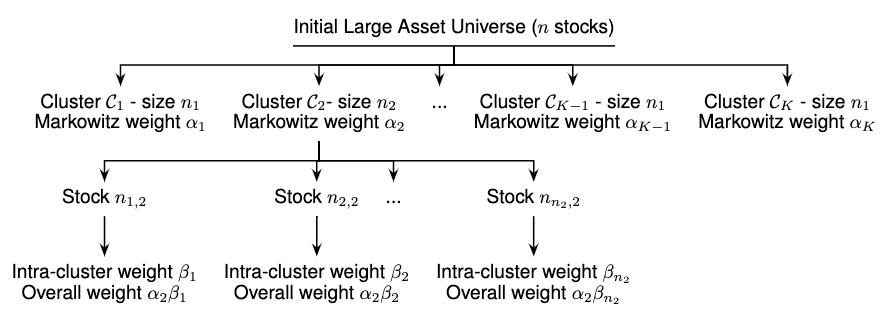
\includegraphics[width=0.80\linewidth]{Source/three.png}
        \vspace{-3mm}
        \caption{Hierarchical representation of the large universe during the portfolio construction phase}
        \label{weights-relationship}
\end{figure*}

\section{Spectral Clustering Algorithms}
\label{spectral-clustering}

Following the description of the graph construction, the focus shifts to the partitioning of the graph based on node correlations. Four algorithms are introduced for this purpose: the spectral clustering algorithm \cite{NIPS2001_801272ee}, the signed Laplacian algorithm \cite{KunegisSL}, the SPONGE algorithm, and its variant, symmetric SPONGE \cite{cucuringuSPONGE}. In the subsequent discussion, let \(\mathcal{G} = (\mathcal{V}, \mathcal{E})\) represent the signed graph constructed as outlined, where \(\mathcal{V} = \{\mathbf{r}^{(1)}, \ldots, \mathbf{r}^{(n)}\}\) denotes the set of nodes and \(\mathcal{E} \subseteq \{\{x, y\} : x, y \in \mathcal{V}\}\) denotes the set of edges. Additionally, \(D\) represents the degree matrix of this graph, \(\Gamma\) is the adjacency matrix, and \(L_N = I - D^{-1/2} \Gamma D^{-1/2}\) is the normalized Laplacian matrix.

\subsection{Spectral clustering algorithm}

In standard spectral clustering, the adjacency matrix typically consists of positive entries. In contrast, the present study retains the adjacency matrix $\Gamma$ of the signed graph, despite the potential for negative entries. This approach is supported by the justification provided in \cite{Knyazev}. It is also consistent with the methodology used by the authors of \cite{SigNet}, whose publicly accessible code is employed in the numerical simulations conducted here. Beyond this modification to the input matrix, the procedure described by Ng et al. in \cite{NIPS2001_801272ee} is followed.

\begin{itemize}
    \item \textbf{Input:} $\Gamma \in \mathbb{R}^{n \times n}$, adjacency matrix of the signed graph, and the number $K$ of clusters;
    \item \textbf{Output:} Clusters $C_1, \ldots, C_K$ partitioning $\{1, \ldots, n\}$.
    \item \textbf{Procedure: }
    \begin{enumerate}
        \item Compute the normalized Laplacian matrix $L_N$;
        \item Compute the $K$ eigenvectors $u_1, \ldots, u_K$ associated with the smallest eigenvalues of $L_N$;
        \item Form the matrix $U$ of size $n \times K$ with columns $u_1, \ldots, u_K$;
        \item Form the matrix $T$ of size $n \times K$ by normalizing the rows of $U$ to have Euclidean norm,
        \begin{align*}
            t_{i,j} = \frac{u_{i,j}}{\sqrt{\sum_{k=1}^K u_{i,k}^2}} \quad  \forall i = 1, \hdots, n \mbox{ and } j = 1, \ldots, K
        \end{align*}
        \item Create clusters $C_1, \ldots, C_K$ on the rows of $T$ using $k$-means++.
    \end{enumerate}
\end{itemize}


\subsection{Signed Laplacian}
This algorithm can be expressed either as an optimization problem on the eigenvectors of $L_N$ or as a minimization problem involving so-called \textit{cut ratios}. In \cite{KunegisSL}, Kunegis et al. decompose the adjacency matrix $\Gamma$ into two matrices, $\Gamma^+$ and $\Gamma^-$, such that $\Gamma = \Gamma^+ - \Gamma^-$, with $\Gamma^+_{ij} > 0$ and $\Gamma^-_{ij} > 0$ (which is equivalent to considering two unsigned subgraphs $\mathcal{G}^+$ and $\mathcal{G}^-$). They then define positive (resp. negative) cuts, denoted $\text{cut}_{\mathcal{G}^+}$ (resp. $\text{cut}_{\mathcal{G}^-})$, that account for positive and negative edges, respectively, associated with a partition $C_1, \ldots, C_k$
\begin{align*}
\begin{cases}
    \text{cut}_{\mathcal{G}^+}(C_1, \ldots, C_k) := \frac{1}{2} \sum_{\ell = 1}^k W^+(C_{\ell}, \overline{C_{\ell}}) \quad\\
    \text{cut}_{\mathcal{G}^-}(C_1, \ldots, C_k) := \frac{1}{2} \sum_{\ell = 1}^k W^-(C_{\ell}, \overline{C_{\ell}}), \\
\end{cases}
\end{align*}
where $W^+(U, V) = \sum_{i \in U, j \in V} \Gamma^+_{ij}$ and $W^-(U, V) = \sum_{i \in U, j \in V} \Gamma^-_{ij}$. 

This leads us to define the following \textbf{signed cut} of a clustering $C_1, \ldots, C_k$ as the quantity $\text{SignedCut}(C_1, \ldots, C_k)$ equal to 
\begin{align*}
2 \text{cut}_{\mathcal{G}^+}(C_1, \ldots, C_k) + \text{cut}_{\mathcal{G}^-}(C_1, \ldots, C_k) + \text{cut}_{\mathcal{G}^-}(C_1, \ldots, C_k),
\end{align*}
% 
and to define the signed ratio cut (SRC) as follows
% 
$$ \text{SRC}(C_1, \ldots, C_k) = \sum_{\ell=1}^k \frac{\text{SignedCut}(C_{\ell}, \bar{C_{\ell}})}{|C_l|}. $$
This allows us to define the signed Laplacian clustering Algorithm 

\begin{itemize}
    \item \textbf{Input:} $\Gamma$, adjacency matrix; $K$ the number  of clusters;
    \item \textbf{Output:} Clusters $C_1, \ldots, C_K$ partitioning $\{1, \ldots, n\}$.
    \item \textbf{Procedure: }
    \begin{enumerate}
        \item Split $\Gamma$ into $\Gamma^+$ and $\Gamma^-$ as previously ;
        \item Find the partition $C_1, \ldots, C_K$ that minimizes the \textbf{SRC} 
        \begin{equation}
            \min \left\{ \text{SRC}(C_1, \ldots, C_K) : C_1, \ldots, C_K \subset \mathcal{V} \text{ s.t. } \bigcup_{\ell=1}^K C_{\ell} = \mathcal{V} \right\}.
            \label{signedratiocut-minimization}
        \end{equation}
    \end{enumerate}
\end{itemize}


\subsection{SPONGE: Signed Positive Over Negative Generalized Eigenvalues}
In \cite{cucuringuSPONGE}, Cucuringu et al. introduced the SPONGE algorithm, a novel formulation to the signed clustering problem that leverages a generalized eigenvalue method. This algorithm has demonstrated superior performance compared to a range of benchmarks, especially in contexts of a high number of clusters 
$K$ or highly sparse graphs. The formulation is defined as follows

\begin{itemize}
    \item \textbf{Input:} $\Gamma$, adjacency matrix; $K$ the number of clusters
    \item \textbf{Output:} Clusters $C_1, \ldots, C_K$ partitioning $\{1, \ldots, n\}$.
    \item \textbf{Procedure: }
    \begin{enumerate}
        \item Split $\Gamma$ into $\Gamma^+$ and $\Gamma^-$ as before.
        \item Find the partition $C_1, \ldots, C_K$ that minimizes the ratio between \textbf{positive cuts} and \textbf{negative cuts} while introducing regularization terms to encourage clusterings that avoid small-sized clusters by solving:
        \begin{equation}
            \min_{C_1,\ldots,C_k} \sum_{i=1}^{k} \frac{\text{cut}_{\mathcal{G}^+}(C_i, \bar{C_i}) + \tau^+ \text{vol}_{\mathcal{G}^-}(C_i)}{\text{cut}_{\mathcal{G}^-}(C_i, C_i) + \tau^- \text{vol}_{\mathcal{G}^+}(C_i)}, 
            \label{SPONGE-min-cut-pb} 
        \end{equation} 
        where $\tau^+, \tau^- > 0$ are regularization parameters, $\text{cut}_{\mathcal{G}}(C, \bar{C})$ is the total weight of edges crossing from $C$ to $\bar{C}$ in graph $\mathcal{G}$, and $\text{vol}_{\mathcal{G}}(C)$ is the total weight of edges inside $C$ in graph $\mathcal{G}$.
    \end{enumerate}
\end{itemize}

Let $L^+$ (resp. $L^-$) and $D^+$ (resp. $D^-$) denote the Laplacian and degree matrices constructed from $\Gamma^+$ (resp. $\Gamma^-$). The solution to \eqref{SPONGE-min-cut-pb} is given by the eigenvectors corresponding to the \( K \) smallest eigenvalues of $\left( L^- + \tau^+ D^+ \right)^{-1/2} \left( L^+ + \tau^- D^- \right) \left( L^- + \tau^+ D^+ \right)^{-1/2}$. In practice, the SPONGE algorithm identifies the $K$ smallest generalized eigenvectors of $(L^+ + \tau^- D^-, L^- + \tau^+ D^+)$. Subsequently, k-means++ clustering is applied to the resulting $K$-dimensional Euclidean space.

\subsection{Symmetric SPONGE}
Furthermore, the Symmetric SPONGE variant of the SPONGE algorithm is employed, utilizing the symmetric graph Laplacian $\bar{L}_{\text{sym}}$. This variant determines the $K$ smallest eigenvectors of the matrix pair $(L^+_{\text{sym}} + \tau^- I, L^-_{\text{sym}} + \tau^+ I)$, where $L^+_{\text{sym}} = (D^+)^{-1/2} L^+ (D^+)^{-1/2}$ and $L^-_{\text{sym}} = (D^-)^{-1/2} L^- (D^-)^{-1/2}$ denote the symmetric Laplacians of $\Gamma^+$ and $\Gamma^-$, respectively. The use of this symmetric Laplacian is particularly beneficial for networks characterized by skewed degree distributions. Theoretical guarantees for the SPONGE family of algorithms, including insights into cluster recovery as influenced by noise and edge sparsity within signed stochastic block models, have been explored by Cucuringu et al. \cite{cucuringuSPONGE}.



\section{Cluster-driven Portfolio Construction and Trading Strategy - Mathematical Framework}
\label{trading-strat}

Having introduced the general problem formulation, the graph construction, and the clustering approach, the next step is to implement a trading strategy that utilizes this portfolio construction methodology to demonstrate its economic advantages. This section will first outline the principles of the strategy and its practical implementation, followed by a discussion of the parameter settings used. 
\vspace{5pt}
\begin{table}[h]
\centering
\begin{tabular}{ll}
\toprule
\textbf{Parameter} & \textbf{Description} \\
\midrule
\textit{Size of the asset universe} & \( n \in \mathbb{N} \) \\
\textit{Number of clusters} & \( K \in \mathbb{N} \) \\
\textit{Lookback window} & \( L \in \mathbb{N} \) \\
\textit{Evaluation window} & \( s \in \mathbb{N} \) \\
\textit{Robustness parameter} & \( R \in \mathbb{N} \) \\
\bottomrule
\end{tabular}
\caption{Summary of main parameters.}
\label{tab:parameters}
\end{table}

\subsection{General setting and procedure}
\label{general-setting-strat}
The trading strategy is decomposed into the four following steps,

\begin{enumerate}
    \item[(i)] \textbf{CLUSTERING}: 
    cluster assets based on historical data returns with a lookback window of $L$ trading days prior to the present day (hence based on $\Tilde{\mathbf{r}}^{(i)} \in \mathbb{R}^L, ~ \forall i \in \{1, \hdots, n\}$).
    \begin{enumerate}
        \item[$\bullet$] \textbf{Input}: asset returns  on $L$ days $\Tilde{\mathbf{r}}^{(1)}, \hdots, \Tilde{\mathbf{r}}^{(i)}$;
        \item[$\bullet$] \textbf{Output}: vector of cluster labels $A \in \mathbb{R}^{n}$ where $A^{(i)} \in \{1, \hdots, K\}$ and $\forall i, ~ \mathbf{r}^{(i)} \in \mathcal{C}_{A^{(i)}}$.
    \end{enumerate}
.
    \item[(ii)] \textbf{PORTFOLIO CONSTRUCTION PHASE}: For each cluster $k \in \{1, \ldots, K\}$, compute the following in order:
    \begin{enumerate}
        \item[(a)] \textit{Intra-cluster weights} \((\beta_{i,k})\), representing the weight of each asset within its cluster (see subsection \eqref{gaussian-weights} for details);
        \item[(b)] The \textit{return} \(r^*_k\) and \textit{expected return} \(\bar{r}^*_k\) of the cluster, where \(r^*_k = \sum_{i=1}^n \beta_{i,k} r_i \mathbf{1}_{(A^{(i)}=k)}\) and \(\bar{r}^*_k = \sum_{i=1}^n \beta_{i,k} \bar{r}_i \mathbf{1}_{(A^{(i)}=k)}\).
    \end{enumerate}

    The \textit{covariance matrix} $\boldsymbol{\Sigma}^*$ for the "cluster" asset universe is defined as $\boldsymbol{\Sigma}^* = (\text{cov}(r^*_k, r^*_l))_{1 \leq k,l \leq K} \in \mathbb{R}^{K \times K}$. \textit{Extra-cluster weights} \(\alpha_1, \ldots, \alpha_K\) are the Markowitz optimal portfolio weights for each cluster, representing the solution to \((\boldsymbol{\mathcal{M}}^*)\) (see \ref{markowitzproblem-cluster}). Consequently, the weight of the \(i\)-th asset in the overall portfolio is \(\alpha_{A^{(i)}} \beta_{i, A^{(i)}}\). The relationships between these weights are illustrated in Figure \ref{weights-relationship}.

    \begin{enumerate}
        \item[$\bullet$] \textbf{Input}: vector of cluster labels $A \in \mathbb{R}^n$;
        \item[$\bullet$] \textbf{Output}: weight vector (\textit{i.e.} portfolio) $\bm{\omega} = [\omega_1, \hdots, \omega_n]^T$, where $\omega_i =\alpha_{A^{(i)}}\beta_{i, A^{(i)}}$ \\
    \end{enumerate}

    \item[(iii)] \textbf{ROBUSTNESS}: Iterate phases (1) and (2) \( R \) times \textit{within the same time frame} \([t-L; t]\) to minimize variability caused by the randomness of clustering methods (\textit{e.g.}, k-means in SPONGE).
    \begin{enumerate}
        \item[$\bullet$] \textbf{Input}: \( R \) portfolios \(\bm{\omega}_1, \ldots, \bm{\omega}_R\) (outputs from phase (2));
        \item[$\bullet$] \textbf{Outcome}: Final portfolio \(\boldsymbol{\omega}_{mean} = \frac{1}{R} \sum_{r=1}^R \bm{\omega}_r \in \mathbb{R}^n\), calculated as the mean of the portfolios across all runs.
    \end{enumerate}
       
    \item[(iv)] \textbf{EVALUATION PHASE}: Initiate the portfolio with long/short positions in each constituent, and hold these positions for the \textit{evaluation window} \([t; t+s]\), where \(s\) is the window length.
\end{enumerate}

At the end of the evaluation window, the procedure is repeated starting at time \( t+s \), with clustering performed on \([t+s-L; t+s]\) and evaluation on \([t+s; t+2s]\). The portfolio positions are then updated based on the newly computed allocations (see Figure 
\ref{sliding-window-representation}).
\begin{figure}[H]
    \centering
    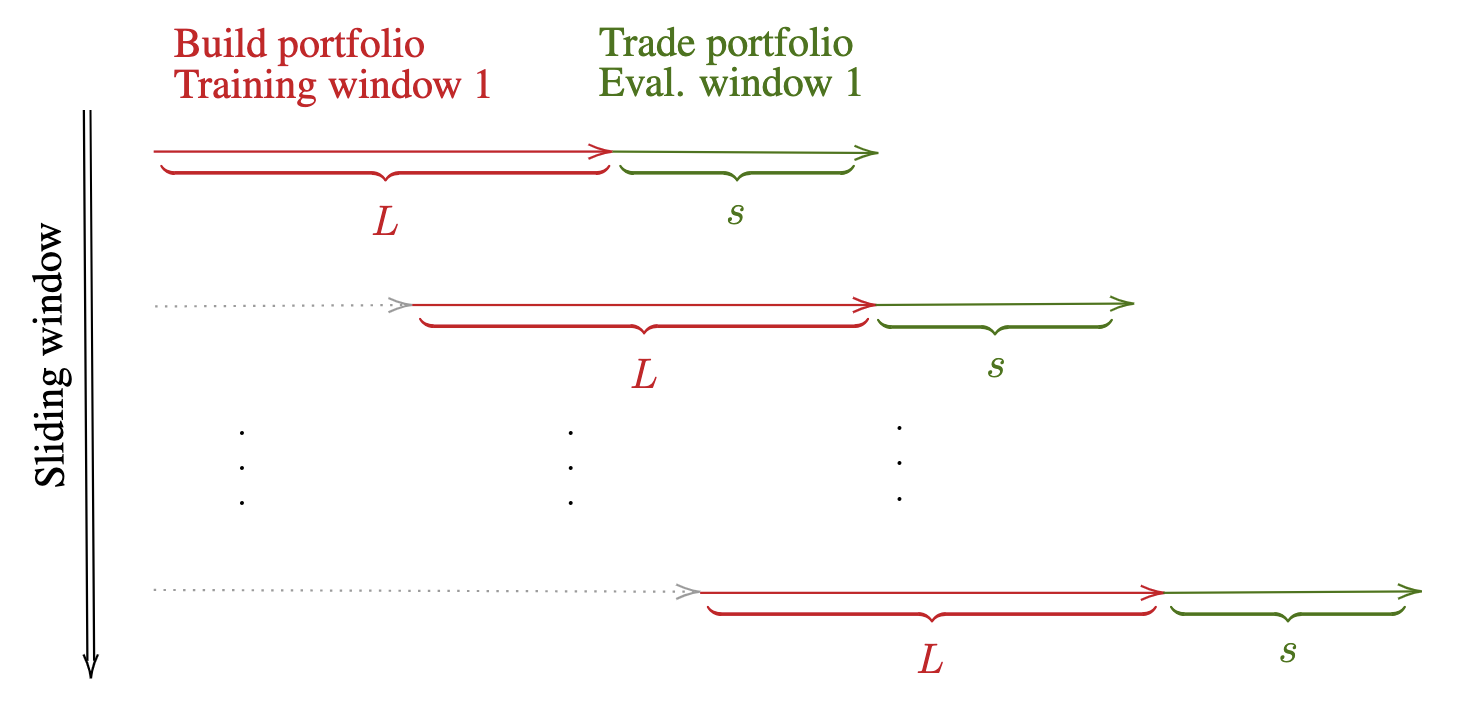
\includegraphics[width=1.0\linewidth]{Source/strat.png}
    \caption{Representation of the walk-forward train-test split of the  strategy.}
    \label{sliding-window-representation}
\end{figure}

\subsection{Gaussian constituent weights}
\label{gaussian-weights}

The \textit{intra-cluster weights} (\(\beta_{i,k}\)) are defined in step (2) as follows. For each cluster \(k\), the weight \(\beta_{i,k}\) of the \(i\)-th asset is calculated as a function inversely proportional to its distance from the cluster center \(\mu_k\). Instead of designating a single representative asset per cluster, this approach ensures that all assets contribute proportionally within their respective clusters. To address the inherent non-linearity in the data, a Gaussian kernel function is employed to derive these similarity weights
$$
\beta_{i_k} = \frac{\exp\left(-\frac{\lVert \mathbf{r}^{(i)} - \mu_k \rVert^2}{2\sigma^2}\right)}{\sum_{j \in \mathcal{C}_k}\beta_{j_k}},
$$
\noindent where $\sigma^2$ is the kernel bandwidth (measuring dispersion) and $\mu_k$ corresponds to the center of the $k$-th cluster defined as the vector containing the mean return of each asset in the cluster. This approach maintains a high level of diversification while accentuating the distinctions between each cluster. Cross-validation on the training window is the approach retained to fix the size of $\sigma^2$.

\subsection{Estimation of returns for Markowitz}
\label{estimation-eta}
The estimation of future returns for each cluster ($\bar{r}^*$ in \eqref{markowitzproblem-cluster}) is crucial, as it significantly impacts the Markowitz weights of the clusters and, consequently, the performance of the portfolio. Since this work does not focus on return forecasting, an indicative procedure is proposed to simulate a forecast, thereby enabling the examination of portfolio performance sensitivity to forecast quality. According to the construction procedure outlined in Section \eqref{general-setting-strat}, assume the portfolio is constructed (and initiated) at time $t$ and held over the period $[t, t+s]$. For each $k \in \{1, \ldots, K\}$, let $\textbf{y}_k \in \mathbb{R}^{s}$ denote the \textit{true} vector of future returns over the $s$ evaluation days, which can be reconstructed from historical data in this experiment. An overall empirical correlation level of $\eta > 0$ is fixed. Since not all assets are equally predictable, the objective is to determine the minimal common noise level $\sigma_{\eta} = [\sigma_{\eta}^{(1)}, \ldots, \sigma_{\eta}^{(s)}] \in \mathbb{R}^{s}$ such that the average empirical correlation (denoted $\widehat{\text{corr}}$) between $\textbf{y}_k$ and its noisy version $\hat{\textbf{y}}_k = \textbf{y}_k + \epsilon_k$, where $\epsilon_i \sim \mathcal{N}(0, \sigma_{\eta}^2 I_s)$, equals $\eta$   

$$
\frac{1}{K}\sum_{k=1}^K\widehat{\text{corr}}(\textbf{y}_k, \hat{\textbf{y}}_k) = \eta. 
$$

To find $\sigma_{\eta}$ for a correlation level $\eta$, the series of returns \textbf{y} for each asset is progressively noised to obtain $\hat{\textbf{y}}$ until the desired correlation is achieved. 

\subsection{Optimal number of clusters}
\label{optimal-number-of-clusters}
The number of clusters, $K$, is a critical parameter that must be determined in advance. To identify its optimal value, the approach described by Cartea et al. \cite{StatisticalArbitrage} is employed. This method involves analyzing the proportion of variance explained by the eigenvalues of the correlation matrix, denoted as $\lambda_1 > \lambda_2 > \ldots > \lambda_n$. A threshold $P \in \mathbb{R}$ is established, and the goal is to determine the smallest integer $k \in \{1, \ldots, n\}$ such that

\begin{align*}
    \frac{\sum_{i=1}^{k} \lambda_i}{\sum_{i=1}^{n} \lambda_i} \geq P. 
\end{align*}
From a principal component analysis perspective, this inequality determines the minimum number $k$ of eigenvalues needed to account for a specified proportion $P$ of the total variance. In this context, $k$ also represents the number of clusters used for partitioning the network.

% \begin{wrapfigure}{r}{0.25\textwidth}
\begin{figure}
    \centering
    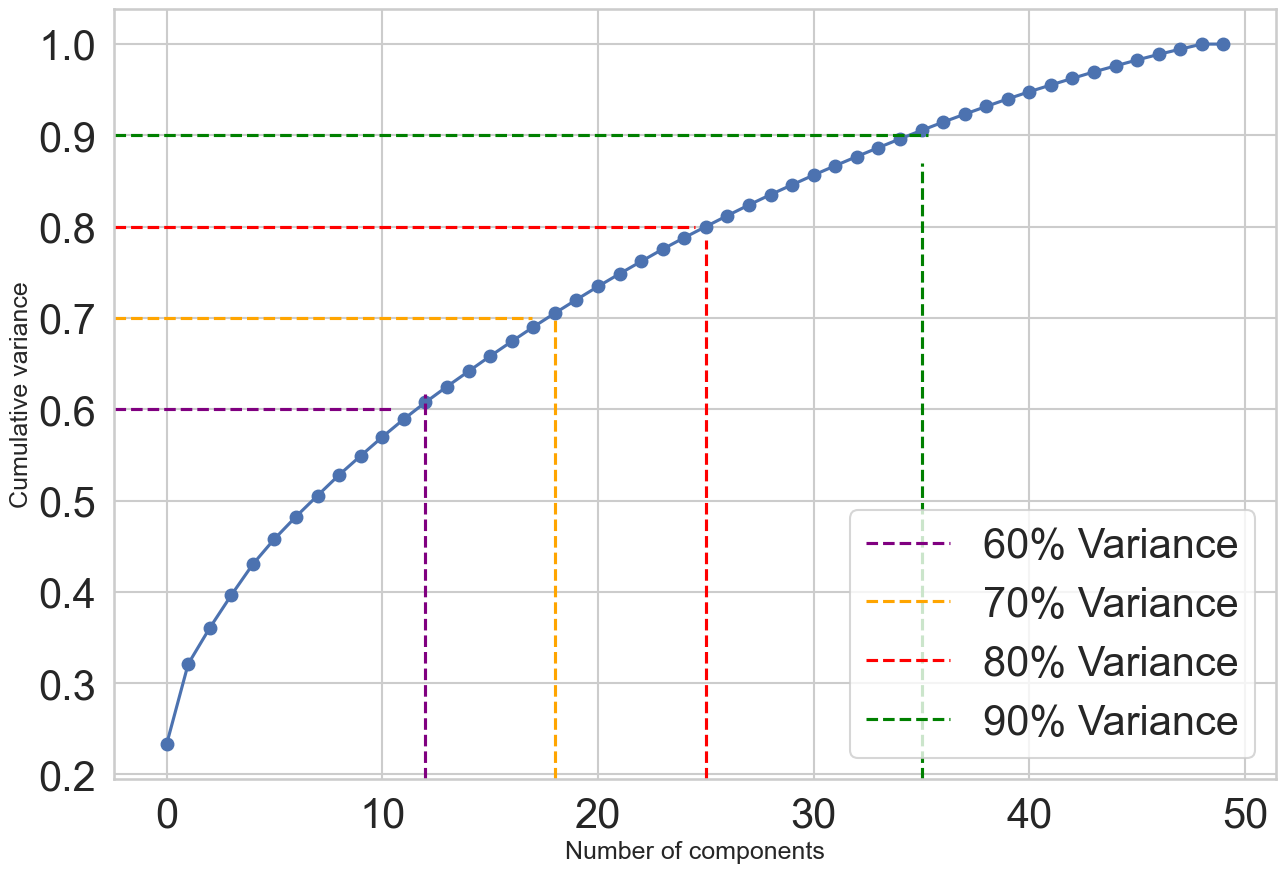
\includegraphics[width=0.4\textwidth]{Source/PCA.png} % Replace 'example-image' with your image file
    \caption{PCA analysis - cumulative variance}
    \label{fig:example}
% \end{wrapfigure}
\end{figure}


Notably, the analysis highlights two prominent numbers of clusters: 10 and 24. These figures correspond to the first two levels of the Global Industry Classification Standard (GICS®): 10 sectors and 24 industry groups. The GICS® framework categorizes the global economy into a hierarchical structure of sectors, industry groups, and sub-industries, and is extensively utilized in the construction of stock indices for assessing global financial market performance.


\subsection{Turnover and transaction costs}

To provide a more realistic yet simple measure of the economic performance of the strategy, linear transaction costs are deducted from the profit and loss (PnL). At the $t$-th trading period, let $V_t$ denote the total portfolio value, and let $\omega_{t,i}$ and $\omega_{t-1,i}$ represent the new and old weights of the $i$-th asset in the portfolio, respectively. The turnover, \textit{i.e.}, the volume of assets exchanged in value, is then given by
$$ TO_t = \sum_{i=1}^{n} |T_{t,i}| = V_t \times \sum_{i=1}^{n} |w_{t,i} - w_{t-1,i}|. $$
A transaction cost $TC_t$ is considered, calculated as $\tau_\text{transac}$\% of the turnover (with $\tau_\text{transac}$ set at 1 basis point in the simulations), such that $TC_t = \tau_\text{transac} \times TO_t$. The net profit and loss (PnL) after accounting for transaction costs is then expressed as follows
\begin{equation}
\text{PnL}_{t, \text{net}} = \text{PnL}_{t, \text{initial}} - TC_t.
\end{equation}
The impact of transaction costs on the performance of the optimal cluster-driven Markowitz strategy is examined (refer to Section \ref{EWA-clustering}), employing SPONGE with 24 clusters and $\eta=0.01$ (indicating a prediction accuracy of 1\%), at both daily and weekly frequencies. The cumulative return of this strategy is compared with that of the naive Markowitz strategy, evaluated without transaction costs.


% \begin{wrapfigure}{r}{0.3\textwidth}
\begin{figure}
    \centering
    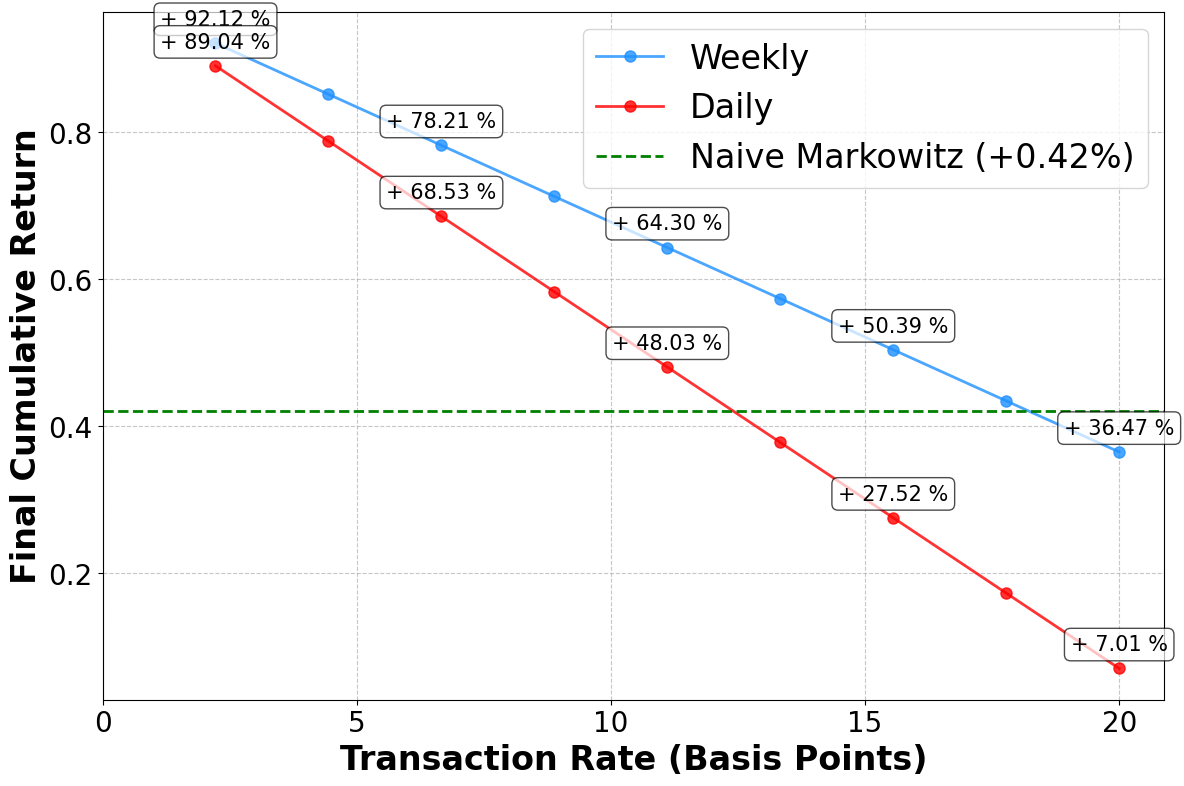
\includegraphics[width=0.43\textwidth]{Source/transac_cost_impact.png} % Replace 'example-image' with your image file
    \caption{Impact of transaction costs on cumulative returns}
    \label{transac-cost-impact}
\end{figure}    
 %\end{wrapfigure}

It is observed in Figure \ref{transac-cost-impact} that transaction costs have a more pronounced impact when applied on a daily basis. Specifically, the daily portfolio outperforms a naive strategy up to approximately 13 basis points, while the weekly portfolio performs better than the naive strategy up to around 18 basis points. It is important to note that for professional traders, transaction costs in US equity markets typically range in the low single digits, often falling below 1 basis point.

\subsection{Exponentially weighted average covariance matrix - the problem of non-stationarity}

Thus far, we have focused on estimates of the uniformly weighted covariance matrices, thus treating each observation equally. However,  empirical finance evidence dating back to \cite{Mandelbrot} suggests that financial returns exhibit certain patterns such as \textit{volatility clustering}, which can skew our observations, effectively reducing the sample size, as returns are dominated by days with significant fluctuations. Consequently, the use of exponentially weighted average (EWA) schemes is arguably more suitable for non-stationary or heteroskedastic environments, as they adjust the effective sample size to incorporate more local observations. The matrix of observations is denoted by $\bm{X} = (\mathbf{r}^{(j)}_i)_{1 \leq i \leq d, 1 \leq j \leq n} = \begin{bmatrix} \mathbf{r}^{(1)} | \hdots |\mathbf{r}^{(n)}\end{bmatrix} \in \mathbb{R}^{d \times n}$ and returns are assumed to be centered (i.e., $\mathbb{E}[\mathbf{r}^{(i)}] = 0$, $\forall i \in \{1, \hdots, n\}$). We then define the EWA sample covariance matrix (referring to \cite{TanZohren}) as 
\begin{equation*}
\bm{E} := \frac{1 - \beta}{1 - \beta^d} \sum_{t=1}^{d} \beta^{d-t} x_t^T x_t \in \mathbb{R}^{n \times n}, 
\end{equation*}
where $x_1, \hdots, x_d \in \mathbb{R}^{1\times n}$ denote the rows of the $\bm{X}$, containing the returns of assets $1, \hdots, n$ during day $t \in \{1, \hdots, d\}$ and  $\beta \in (0, 1)$ denoting the \textit{exponential decay rate}. In the limit where $\beta$ tends to one from below, the EWA converges towards the standard sample covariance; conversely, if $\beta$ moves away from one, it places more weight on the recent cross-product observations.


\section{Empirical results}
\label{empirical}

The framework outlined in Section \ref{trading-strat} is subjected to back-testing on a large universe of assets of $n=695$ stocks for which we have daily data available every day for the entire duration of the study (refer to database \cite{WhartonDATA}, which includes daily returns of NYSE stocks from January 2013 to December 2019). The four trading strategies—named after the respective clustering algorithms—are compared with each other as well as with so-called \textit{naive} strategies. These strategies are highly sensitive to their underlying parameters, specifically $\eta$, representing prediction quality, and $K$, the number of clusters. The back-testing is conducted by simulating a portfolio that initially invested \$1 on January 1, 2013, with \$1 reinvested at each trading period based on the evaluation window. In all subsequent simulations, parameter values are fixed as detailed in Table \ref{params}. The number of clusters, \( K \), and the prediction level, $\eta$, are varied across the sets $K \in \{10, 17, 24\}$ and $\eta \in \{0, 0.01, 0.1, 0.5, 0.9, 1\}$, respectively, to evaluate the sensitivity of the strategy to these parameters.

\vspace{3pt}
\begin{table}[H]
  \caption{Table of parameters}
  \label{params}
  \begin{tabular}{cccccccl}
    \toprule
     &  Lookback & $\sigma$ & Repetitions &  Eval. & $\beta$ \\
    \midrule
     & 75 trading days & 0.01 & 10 & 5 trading days& $0.9$ \\
  \bottomrule
\end{tabular}\\
\end{table}

 

\subsection{Naive strategies}


In this section, three naive portfolio construction strategies that do not employ clustering are introduced. These strategies are designed to emphasize the significance of incorporating clustering into the correlation matrix prior to portfolio optimization. Let $n$ represent the number of assets in the universe. The strategies are defined as follows 
\begin{enumerate}
    \item[(i)] \textbf{Equally-weighted portfolio strategy}, denoted by $(\boldsymbol{\omega}_{\text{EW}, t})_t$ and defined by uniform weights \textit{i.e.}
    $$
    (\boldsymbol{\omega}_{\text{EW}, t})_i = \frac{1}{n}, \quad \forall i \in \{1, \hdots, n \}.
    $$
    \item[(ii)] \textbf{Naive Markowitz strategy}, denoted by $(\boldsymbol{\omega}_{\text{MN}, t})_t$ and defined by weights satisfying at each time $t$ 
    $$
    (\boldsymbol{\omega}_{\text{MN}, t})_t \in \underset{\boldsymbol{\omega} \in \mathbb{R}^n}{\arg \min} \left\{\boldsymbol{\omega}^T\boldsymbol{\Sigma}_t \boldsymbol{\omega} : \boldsymbol{\omega}^T \bar{r}_t  \geq \rho_{0}, \sum_{i=1}^n \omega_i = 1\right\}
    $$
    \item[(iii)] \textbf{SP 500 index strategy}, denoted by $(\boldsymbol{\omega}_{\text{SP500}, t})_t$, which consists in holding a long position in an ETF that replicates the SP 500 index.
\end{enumerate}

The evolution of their respective cumulative PnL is given in Figure \ref{naivestrats-plots}.

\begin{figure}[H]
    \centering
    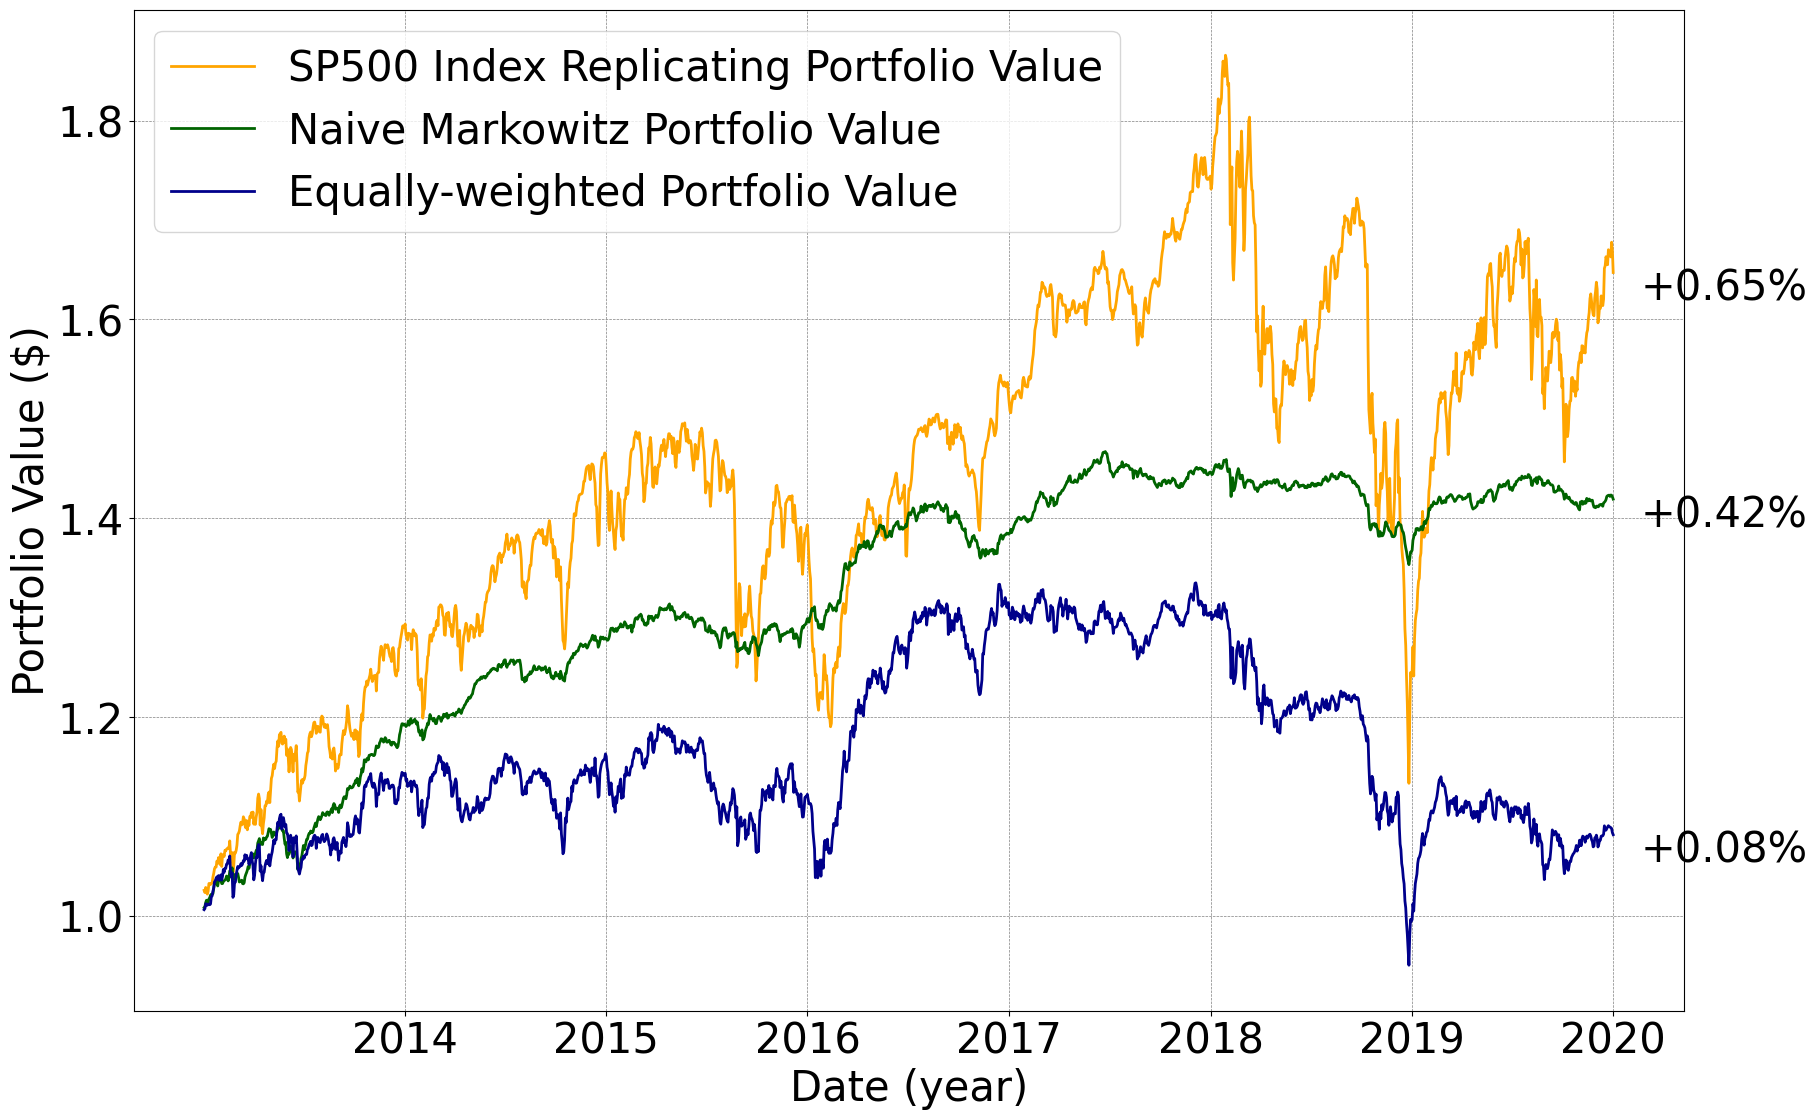
\includegraphics[width=0.9\linewidth]{Source/naive_strats.png}
    \caption{Naive Portfolio Values for 1\$ Initial Investment (01-01-2013 | 31-12-2019)}
    \label{naivestrats-plots}
\end{figure}

We provide the following observations on these results:
\begin{itemize}
    \item[-] In our experimental setting, the uniform strategy performs the worst. However, there have been others lines of work in the literature such as \cite{optimal_perf_good} and \cite{optimal_porfolio_good_perf_2} which claim that equally weighted strategies often outperform more complex models.
    \item[-] The SP 500 replication strategy yields the best returns but at the cost of high volatility, resulting in a Sharpe ratio of 0.5.
    \item[-] Despite the SP 500 losing over 40\% of its value at the end of 2018, the naive Markowitz approach performed well during this downturn.
\end{itemize}


\subsection{Clustering EWA strategies}
\label{EWA-clustering}

The performance of the four cluster-driven Markowitz strategies is compared with that of the naive Markowitz strategy. Figure \ref{cumpnlstrategiesandewa} illustrates the cumulative profit and loss (PnL), while Table \ref{EWA_24_perf_metrics} provides a detailed performance assessment of the EWA-clustering portfolio across various metrics. The cluster-based strategies consistently demonstrate superior economic performance compared to the naive approach.

\begin{figure}[H]
    \centering
    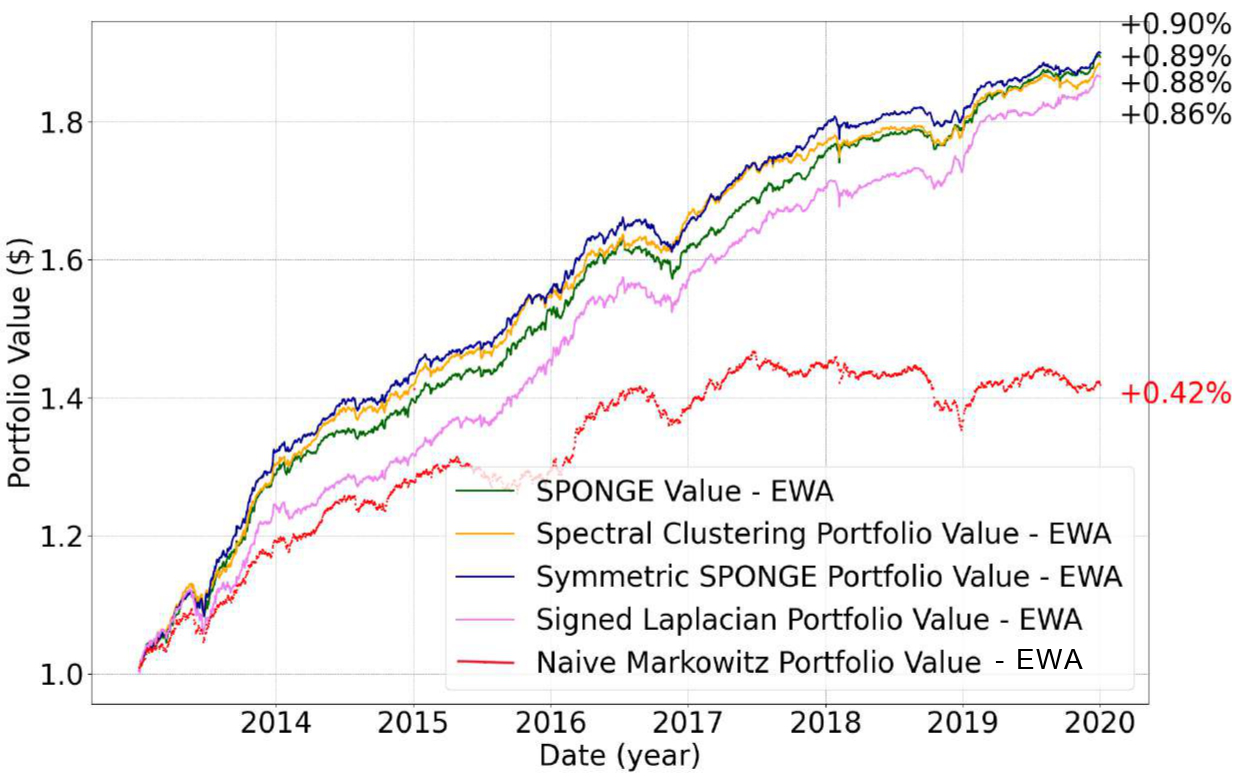
\includegraphics[width=0.9\linewidth]{Source/EWA_strats.png}
    \caption{EWA portfolio clustering values vs. the naive Markowitz portfolio - 24 clusters.}
    \label{cumpnlstrategiesandewa}
\end{figure}


% In this graph, we considered the parameters given in the  table~\ref{tab:parameter-table4}.



\begin{itemize}
    \item[-] \textbf{In terms of volatility}, as measured by annualized and daily volatility, the naive Markowitz strategy performs the worst. Covariance estimation in a lower dimension improves performance.
    \item[-] \textbf{In terms of PnL returns}, measured by Return and Annualized Return (AR), the clustering strategies significantly outperform the naive strategies, even in bear market conditions (\textit{i.e.}, during periods of declining stock prices).
\end{itemize}


These observations lead to the conclusion that the cluster-driven portfolio construction methods, which include EWA, effectively reduce volatility and mitigate risk exposure. The advantageous balance between return and risk is particularly evident when examining Sharpe ratios. Notably, the symmetric SPONGE strategy achieves the highest Sharpe ratio of $3.52$ (see Table \ref{EWA_24_perf_metrics}), signifying that each unit of risk taken yields an average excess return exceeding three units relative to a risk-free investment.
\vspace{3pt}
\begin{table}[H]
  \caption{Performance metrics - EWA - 24 Clusters}
  \label{EWA_24_perf_metrics}
  \begin{tabular}{cccccl}
    \toprule
     &  Naïve & \textbf{SPONGE} &  Sym & SL & SC\\
    \midrule
    Return & \textcolor{red}{41.92\%} & 89.36\% & 89.98\% & 86.45\% &\textcolor{blue}{91.25\%}\\ 
    AR & \textcolor{red}{5.14\%} & 9.57\% & 9.62\% & 9.33\% & \textcolor{blue}{9.73\%} \\ 
    Daily Vol. &  \textcolor{red}{0.23\%} & 0.19\% &  \textcolor{blue}{0.17\%} & 0.22\% & 0.19\% \\ 
    Annual. Vol. &  \textcolor{red}{3.59\%} & 3.09\% &  \textcolor{blue}{2.73\%} & 3.42\% &3.04\%\\ 
    Sharpe & \textcolor{red}{1.43} & 3.09 & \textcolor{blue}{3.52} & 2.72 &3.19\\ 
    Sortino & \textcolor{red}{1.97} & 4.28 & \textcolor{blue}{4.99} & 3.68& 4.33\\ 
  \bottomrule
\end{tabular}
\end{table}

\subsection{Performances sensitivity to the number of clusters}

The sensitivity of the strategy’s performance to the number of asset clusters is now assessed, with all other parameters held constant as specified in Table \ref{params}. Following the analysis in Section \ref{optimal-number-of-clusters}, three cases are considered $K \in \{10, 17, 24\}$, excluding EWA. These values of $K$ are informed by the \textbf{GICS®} classification, suggesting that the cluster-driven strategies may be construed as sectorial asset trading strategies, subdividing the portfolio according to these classifications. The cumulative PnL for these cluster configurations is illustrated in Figures ~\ref{10-clusters}, ~\ref{17-clusters}, ~\ref{24-clusters}. Several observations on the results are detailed below.


\begin{figure}
\centering
\begin{subfigure}{0.9\linewidth}
  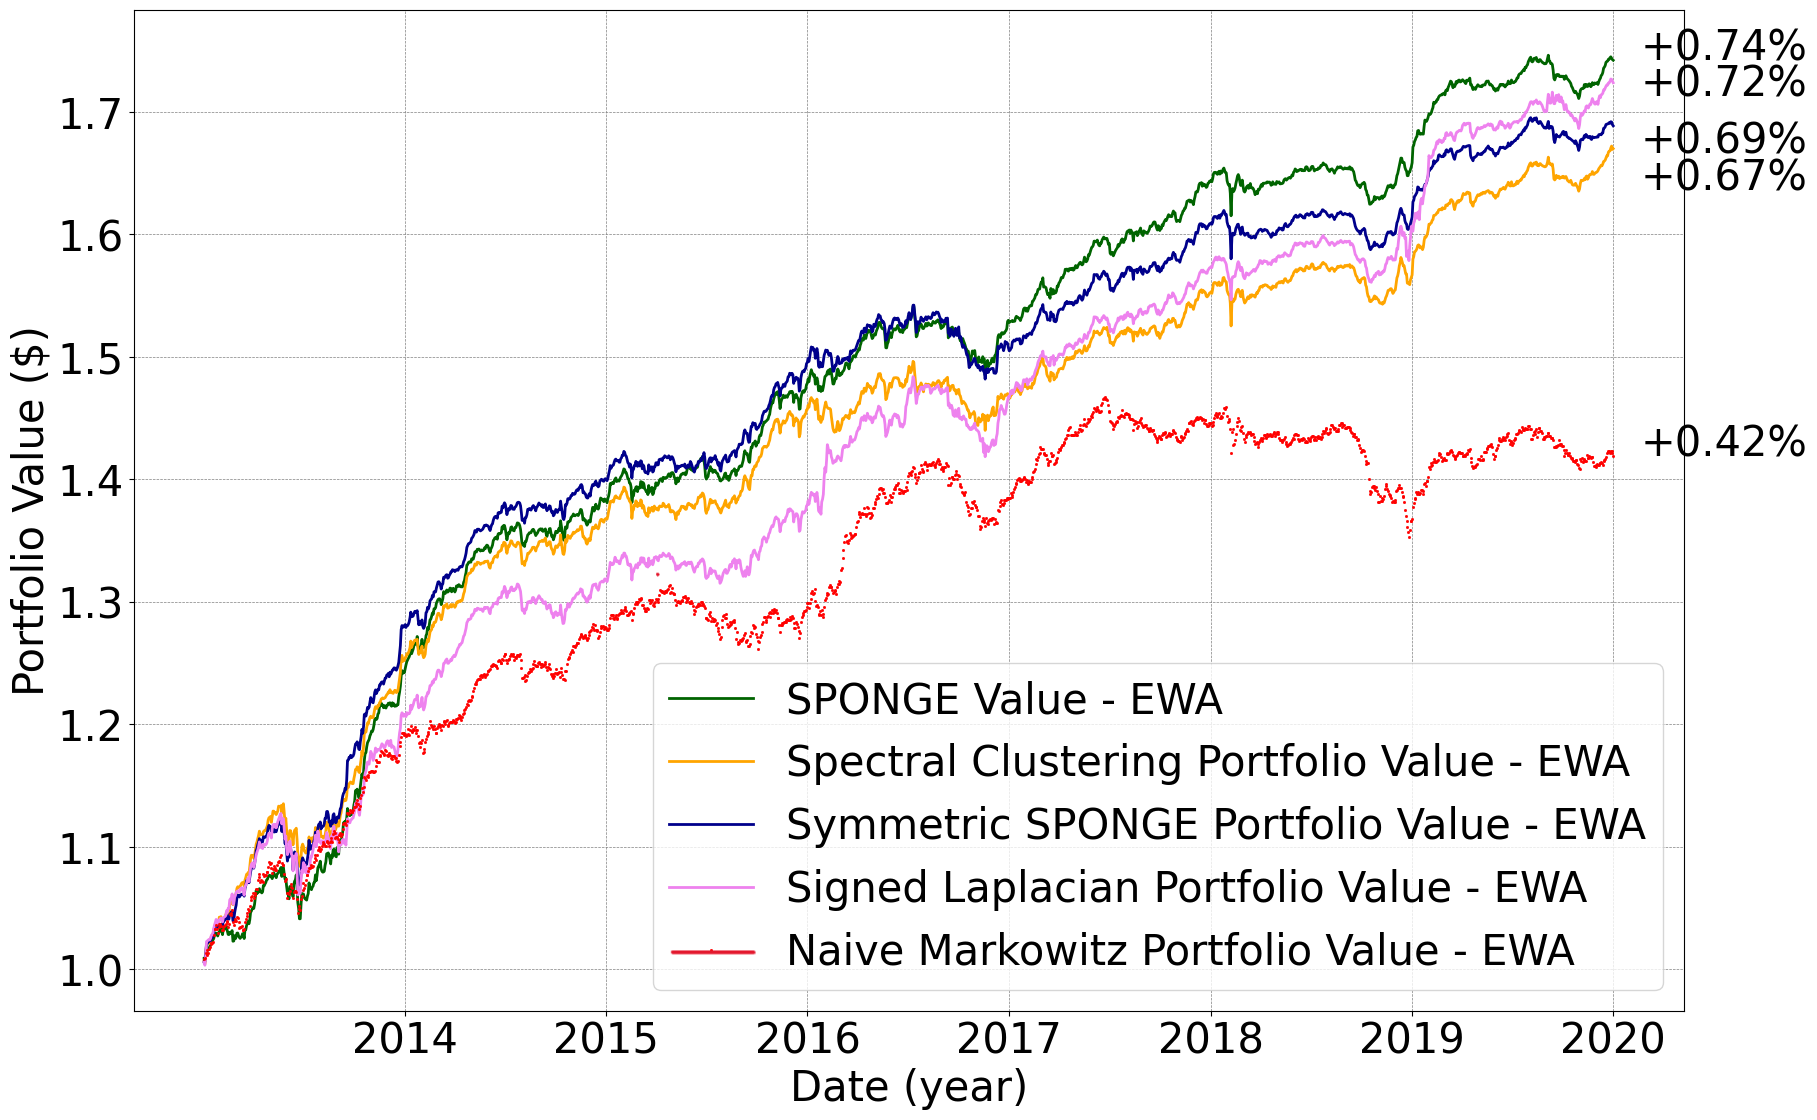
\includegraphics[width=1.0\linewidth]{Source/10_clusters_all.png}
  \caption{$K=10$}
  \label{10-clusters}
\end{subfigure}\hfill
\begin{subfigure}{0.9\linewidth}
  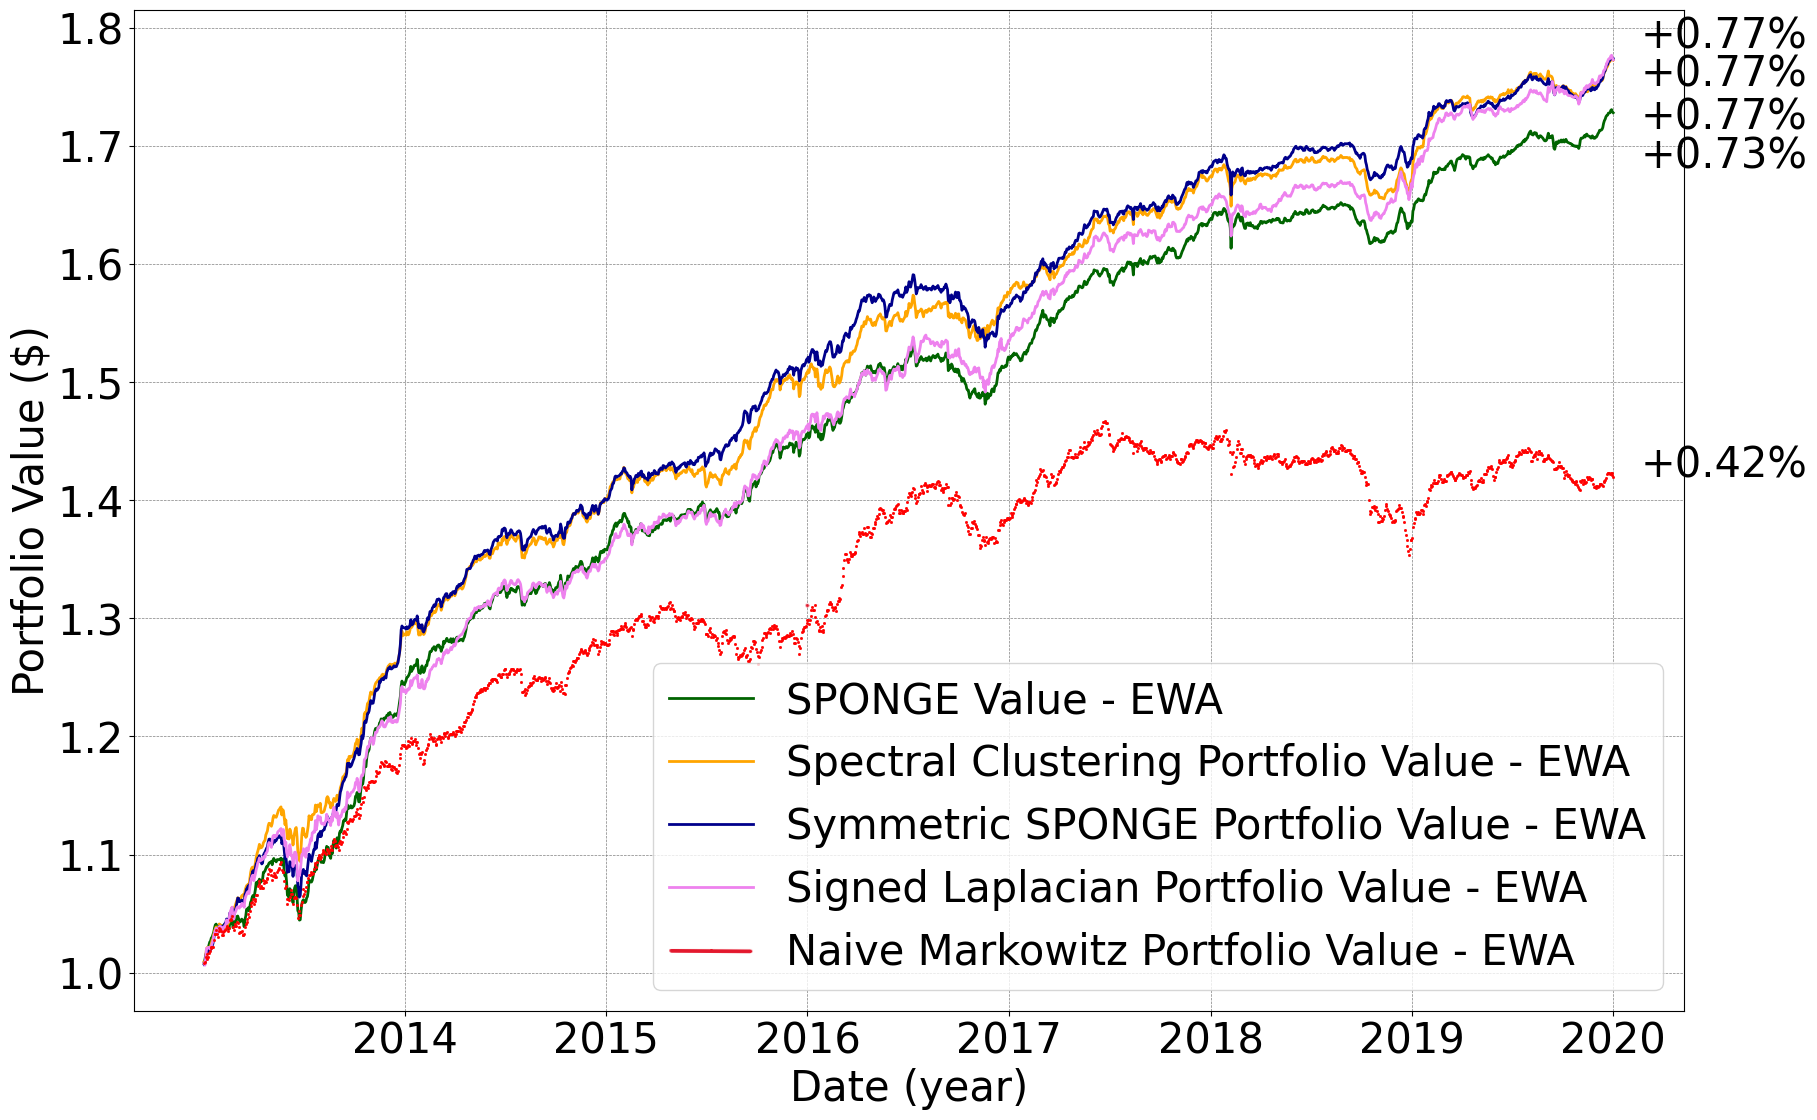
\includegraphics[width=1.0\linewidth,]{Source/17_clusters_all.png}
  \caption{$K=17$}
  \label{17-clusters}
\end{subfigure}
\begin{subfigure}{0.9\linewidth}
  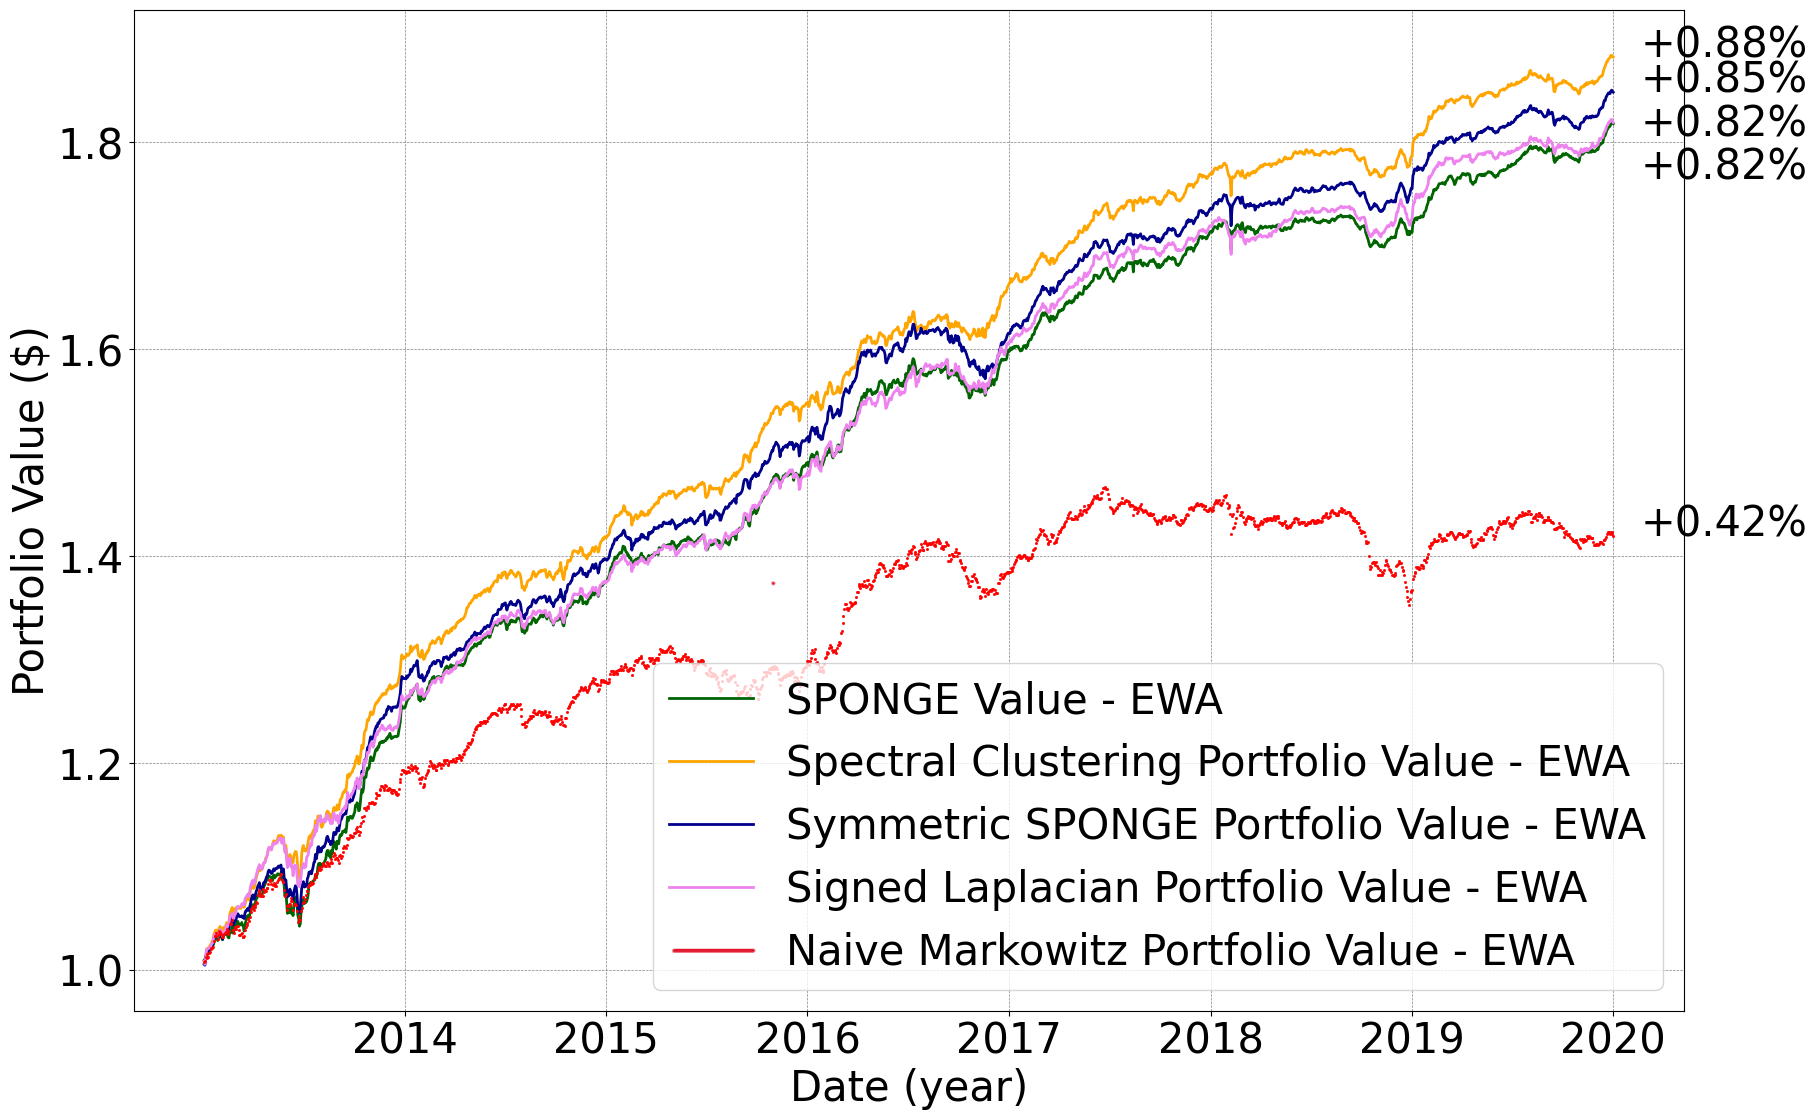
\includegraphics[width=1.0\linewidth]{Source/24-clusters.png}
  \caption{$K=24$}
  \label{24-clusters}
\end{subfigure}
\caption{Portfolio clustering performance for varying $K$}
\end{figure}

\begin{itemize}
    \item[-] Excluding the EWA scheme results in nearly a 10\% reduction in total return (see Figure \ref{24-clusters} compared to Figure \ref{cumpnlstrategiesandewa}).
    \item[-] For $K = 10$, the relatively poor results may be due to significant information loss from extensive dimensionality reduction.
    \item[-] For $K=17$, performance shows slight improvement but may be influenced by limited economic interpretation
    \item[-] For $K=24$, the strategy yields the best results in terms of both return and volatility. This superior performance is likely due to the clear economic rationale behind the 24 clusters (24 industry groups in the GICS®), and the retention of a sufficiently high-dimensional correlation matrix that better preserves information.
\end{itemize}



\subsection{Performance sensitivity to the quality of the prediction ($\eta$)}

The impact of varying $\eta$ is now examined (refer to Section \ref{estimation-eta}). Intuitively, as $\eta$ increases, the empirical correlation between the \textit{true} vector of expected returns and its noisy counterpart also increases, enhancing the quality of predictions. This analysis aims to illustrate how the performance of a strategy might evolve with forecast accuracy. As depicted in Figure \ref{varying-eta} and in Table \ref{varying-eta-table}, improved prediction accuracy leads to enhancements in both returns and volatility, with an extreme case with a perfect prediction $\eta = 1$. Additionally, the case where 
$\eta=0$ meaning the expected return vector is simply the average returns from the training period, is considered. Figure \ref{no-eta} shows the cumulative PnL for this scenario, which results in poorer performance in terms of returns and volatility, although it still achieves a Sharpe ratio above 1. The clustering strategies demonstrate better volatility and higher returns compared to the naive Markowitz approach. 
\vspace{3pt}
\begin{figure}[H]
\centering
\begin{subfigure}{0.9\linewidth}
  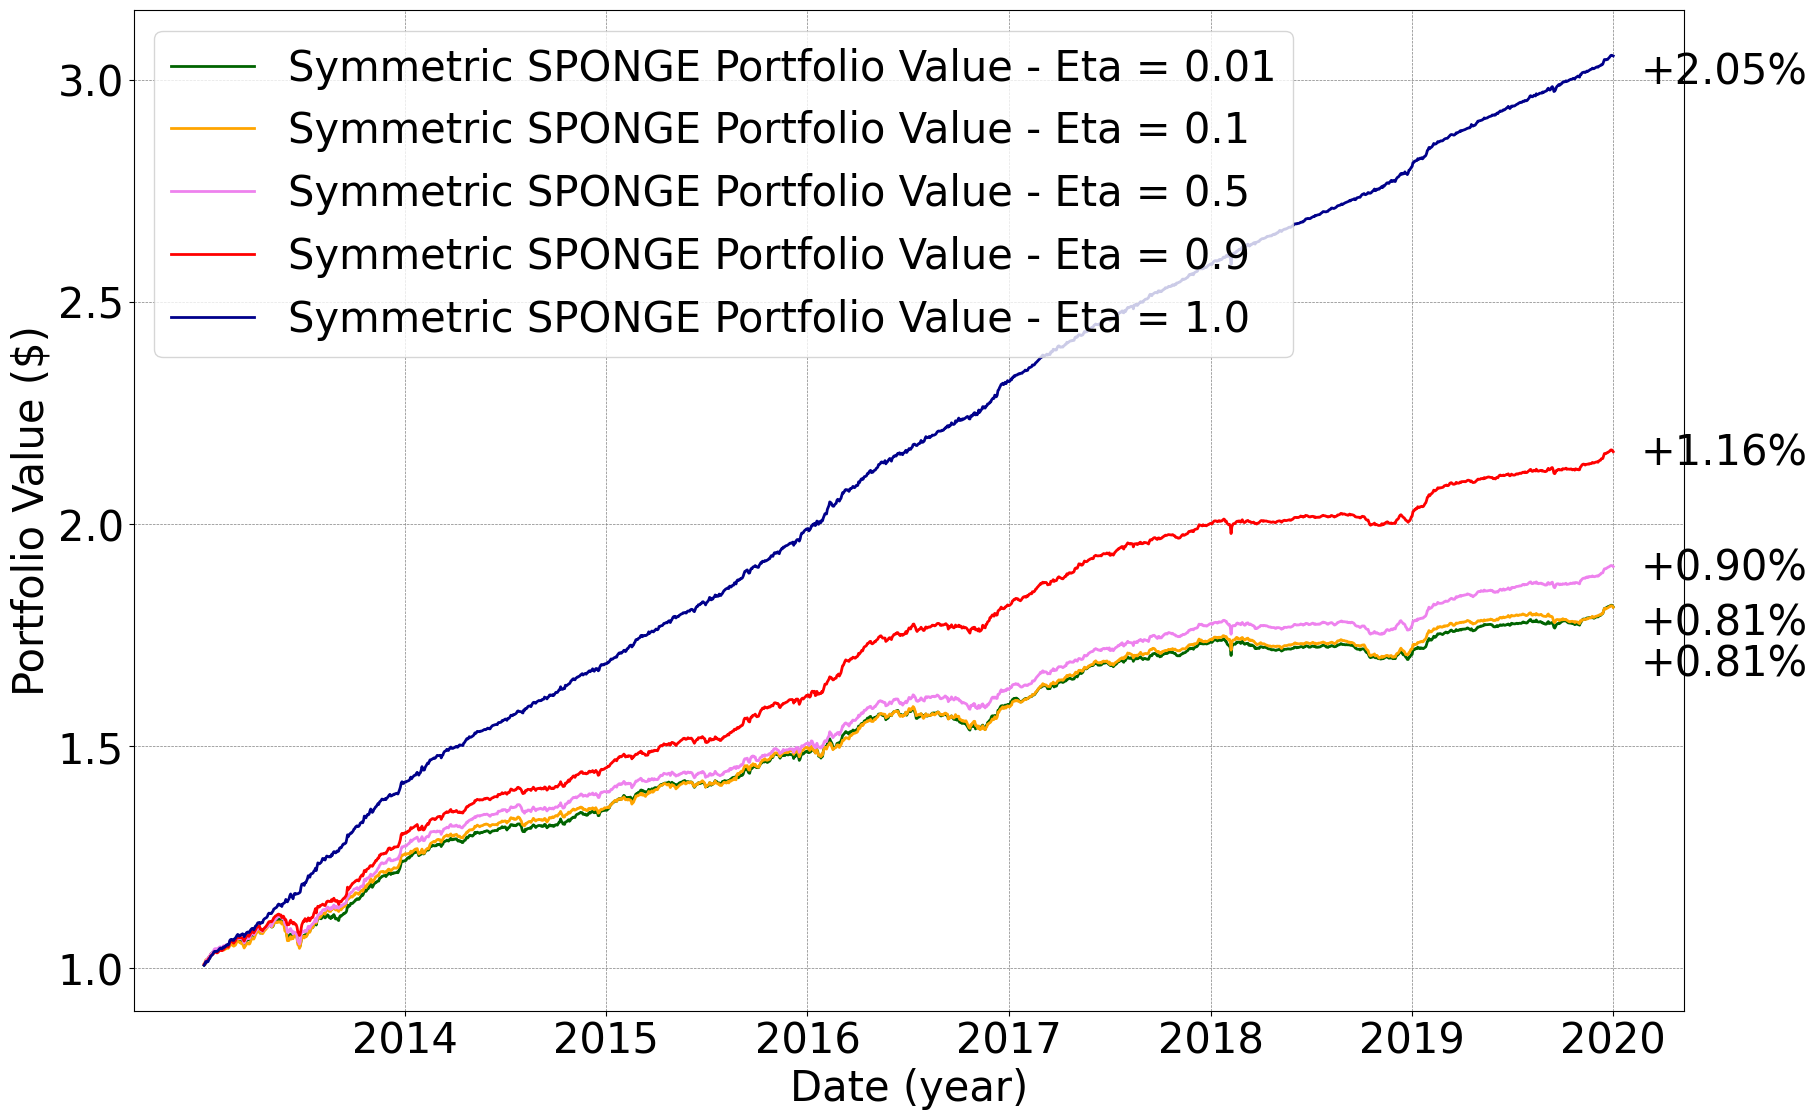
\includegraphics[width=1.0\linewidth]{Source/sponge_sym_eta_varying.png}
  \caption{$\eta \in \{0.01, 0.1, 0.5, 0.9, 1.0\}$}
  \label{varying-eta}
\end{subfigure}\hfill
\begin{subfigure}{0.9\linewidth}
  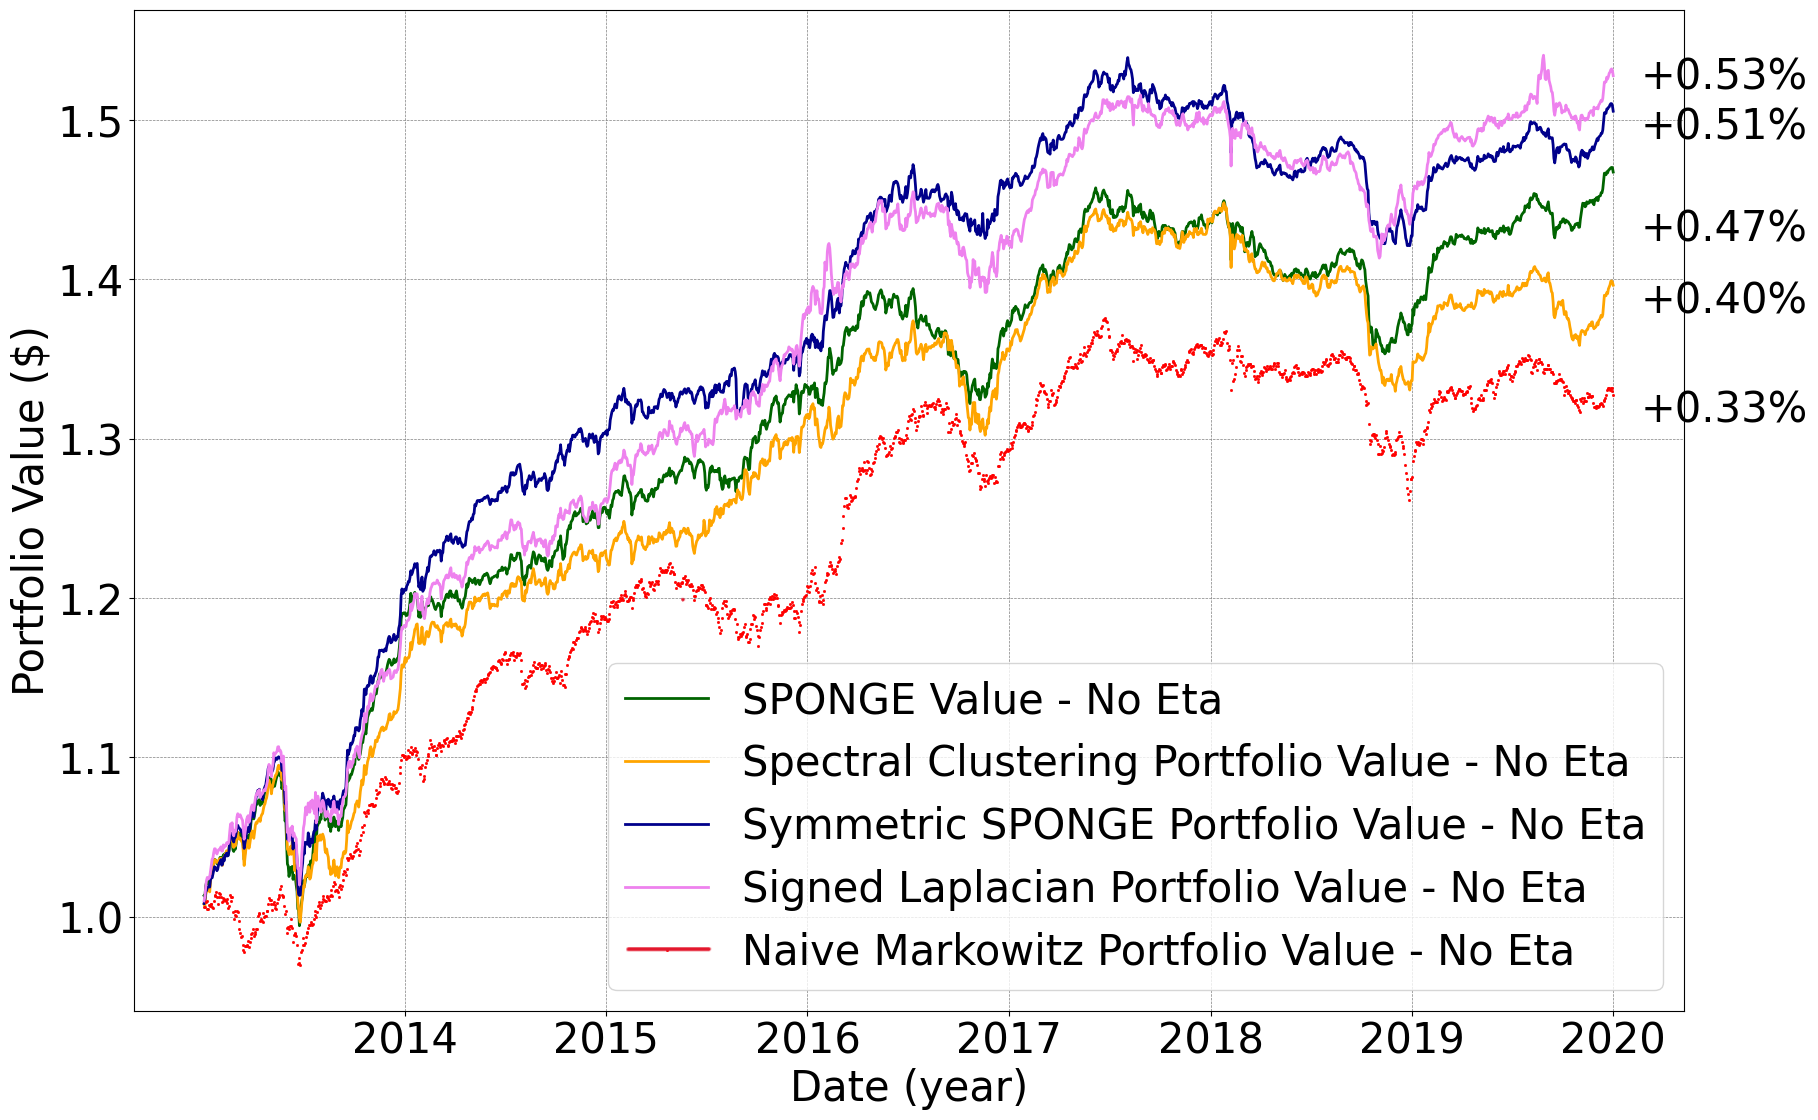
\includegraphics[width=1.0\linewidth]{Source/No_eta_comparison.png}
  \caption{$\eta = 0$}
  \label{no-eta}
\end{subfigure}
\caption{Portfolio clustering values depending on the quality of the prediction $\eta$}
\end{figure}


\begin{table}[H]
  \caption{Perfomance metrics of portfolios - variations of $\eta$}
  \label{varying-eta-table}
  \begin{tabular}{cccccl}
    \toprule
     &  $\eta = 0.01$ & $\eta = 0.1$ &  $\eta = 0.5$ & $\eta = 0.9$ & $\eta = 1.0$\\
    \midrule
    Return & 81.39\% & \textcolor{red}{81.29\%} & 90.47\% & 116.34\% & \textcolor{blue}{205.43\%}\\
    AR & 8.90\% & \textcolor{red}{8.89\%} & 9.66\% & 11.68\% & \textcolor{blue}{17.33\%} \\
    Daily Vol. & \textcolor{red}{0.19\%} & \textcolor{red}{0.19\%} & 0.18\% & 0.17\% & \textcolor{blue}{0.14\%} \\
    Annual. Vol. & 3.04\% & \textcolor{red}{3.09\%} & 2.94\% & 2.76\% &\textcolor{blue}{2.23\%}\\
    Sharpe & 2.93 & \textcolor{red}{2.88} & 3.28 & 4.24 &\textcolor{blue}{7.76}\\
    Sortino & 3.89 & \textcolor{red}{3.75} & 4.58 & 6.00& \textcolor{blue}{12.32}\\
  \bottomrule
\end{tabular}
\end{table}

%\begin{figure}[H]
%    \centering
%    \includegraphics[width=1\linewidth]{PLOTS/plotwithoutalpha.png}
%    \caption{Comparison of naive strategies and three clustering strategies without alpha}
%    \label{fig:enter-label}
%\end{figure}

\vspace{-2mm}
\section{Conclusion}
\label{conclusion}

In this work, we introduced an alternative framework for portfolio construction that leverages graph clustering algorithms to address the complexities of Markowitz Mean-Variance Optimization in large asset universes. To test this method, we built a backtesting framework that revealed compelling results. In terms of Sharpe ratio, the portfolio strategies are ranked, starting from the best one, as follows: Markowitz clustering with EWA, Markowitz with clustering but without EWA, naïve Markowitz portfolio, SP 500 Index and equally weighted portfolio. Using the symmetric SPONGE clustering algorithm, this combination achieves a Sharpe ratio of $3.52$ and a Sortino ratio of $4.99$. These performances demonstrate that while Markowitz optimization is effective in reducing portfolio volatility, it becomes more efficient when coupled with a clustering method to reduce dimensionality, and a better estimation of the covariance to address non-stationary issues inherent in the time series of returns. Under market stress, our portfolio strategy continues to perform well, such as in 2018 when the SP 500 lost more than $40$\% of its value, and our portfolio strategy still showed positive returns. Another interesting finding is that the cluster-driven portfolios perform best with $K=24$ clusters, which could be aligned with its economic interpretation, as there are $24$ industry groups within GICS®, and the fact that the dimensionality remains quite high, preserving more effectively the information content. 

While our research centers on comparing the performance of our clustering and forecasting-based strategy against traditional Markowitz optimization, our framework is highly versatile and can be tailored with various parameters, including different target returns, alternative optimization methods, and diverse constituent weights. Future exploration of these configurations could further improve the effectiveness of the strategy under varying market conditions. 

Looking ahead, several avenues for improvement are worth considering. For the graph construction component, exploring alternative correlation metrics could lead to different covariance matrix estimates. Additionally, examining various clustering methods might provide further insights, as our results indicate that clustering efficiency varies across different scenarios. Incorporating Markowitz optimization within clusters for determining internal weights could integrate our approach with those suggested by \cite{León}, \cite{Tola} and \cite{Gatta}, potentially further enhancing performance. Moreover, leveraging advanced covariance forecasting techniques (see \cite{zhang2022graphCov,gnn2023graphCov}, and also  \cite{CaoZheng} for a method and a review), and enhancing EWA with cross-validation approaches (see \cite{TanZohren}), GARCH models, or deep learning methods, could offer further improvements to our proposed trading strategy. 


\vspace{0mm}

%% The next two lines define the bibliography style to be used, and
%% the bibliography file.
\bibliographystyle{ACM-Reference-Format}
\bibliography{sample-base}

\end{document}
\endinput
%%
%% End of file `sample-sigconf.tex'.
